%%%%%%%% ICML 2025 EXAMPLE LATEX SUBMISSION FILE %%%%%%%%%%%%%%%%%

\documentclass{article}

% Recommended, but optional, packages for figures and better typesetting:
\usepackage{microtype}
\usepackage{graphicx}
\usepackage{capt-of}
\usepackage{subfigure}
\usepackage{multirow}
\usepackage{xcolor}
\usepackage{booktabs} % for professional tables

% hyperref makes hyperlinks in the resulting PDF.
% If your build breaks (sometimes temporarily if a hyperlink spans a page)
% please comment out the following usepackage line and replace
% \usepackage{icml2025} with \usepackage[nohyperref]{icml2025} above.
\usepackage{xurl}
\usepackage[hypertexnames=false]{hyperref}
\usepackage{enumitem}

% Attempt to make hyperref and algorithmic work together better:
\newcommand{\theHalgorithm}{\arabic{algorithm}}

% Use the following line for the initial blind version submitted for review:
% \usepackage{icml2025}

% If accepted, instead use the following line for the camera-ready submission:
\usepackage{icml2025}
\renewcommand{\icmlruler}[1]{}

% For theorems and such
\usepackage{amsmath}
\usepackage{amssymb}
\usepackage{mathtools}
\usepackage{amsthm}
\usepackage[most]{tcolorbox}

\definecolor{findingblue}{HTML}{245A81}
\definecolor{findingbg}{HTML}{F0F6FA}
% if you use cleveref..
\usepackage[capitalize,noabbrev]{cleveref}

%%%%%%%%%%%%%%%%%%%%%%%%%%%%%%%%
% THEOREMS
%%%%%%%%%%%%%%%%%%%%%%%%%%%%%%%%
\theoremstyle{plain}
\newtheorem{theorem}{Theorem}[section]
\newtheorem{proposition}[theorem]{Proposition}
\newtheorem{lemma}[theorem]{Lemma}
\newtheorem{corollary}[theorem]{Corollary}
\theoremstyle{definition}
\newtheorem{definition}[theorem]{Definition}
\newtheorem{assumption}[theorem]{Assumption}
\theoremstyle{remark}
\newtheorem{remark}[theorem]{Remark}

% Todonotes is useful during development; simply uncomment the next line
%    and comment out the line below the next line to turn off comments
%\usepackage[disable,textsize=tiny]{todonotes}
\usepackage[textsize=tiny]{todonotes}


% The \icmltitle you define below is probably too long as a header.
% Therefore, a short form for the running title is supplied here:
\newcommand{\papertitle}{What Remains of Teacher Supervision? An Empirical Study of On-Policy Distillation}
\icmltitlerunning{What Remains of Teacher Supervision?}


% Float-specific caption spacing; the ICML page geometry is unchanged.
\usepackage{etoolbox}
\usepackage{placeins}
\usepackage[all]{hypcap}
\setcounter{dbltopnumber}{2}
\setcounter{topnumber}{6}
\setcounter{bottomnumber}{4}
\setcounter{totalnumber}{8}
\renewcommand{\topfraction}{0.95}
\renewcommand{\bottomfraction}{0.9}
\renewcommand{\floatpagefraction}{0.65}
\renewcommand{\dblfloatpagefraction}{0.65}
\renewcommand{\dbltopfraction}{0.9}
\renewcommand{\textfraction}{0.08}
\setlength{\dbltextfloatsep}{12pt plus 2pt minus 2pt}
\setlength{\dblfloatsep}{7pt plus 2pt minus 2pt}
\clubpenalty=10000
\widowpenalty=10000
\AtBeginEnvironment{table}{\setlength{\abovecaptionskip}{8pt}\setlength{\belowcaptionskip}{5pt}}
\AtBeginEnvironment{table*}{\setlength{\abovecaptionskip}{8pt}\setlength{\belowcaptionskip}{5pt}}
\AtBeginEnvironment{figure}{\setlength{\abovecaptionskip}{6pt}\setlength{\belowcaptionskip}{0pt}}
\AtBeginEnvironment{figure*}{\setlength{\abovecaptionskip}{6pt}\setlength{\belowcaptionskip}{0pt}}


\definecolor{findingborder}{RGB}{90,112,133}
\definecolor{findingbackground}{RGB}{246,248,250}
\newcommand{\findingbox}[2]{%
\par\addvspace{8pt}\noindent
\begingroup\setlength{\fboxsep}{7pt}\setlength{\fboxrule}{0.5pt}%
\fcolorbox{findingborder}{findingbackground}{%
\begin{minipage}{\dimexpr\linewidth-2\fboxsep-2\fboxrule\relax}
\small\textbf{Key Finding #1.} #2
\end{minipage}}\endgroup\par\addvspace{8pt}}

\begin{document}

\twocolumn[
\icmltitle{\papertitle}

\icmlsetsymbol{@anon}{}
\begin{icmlauthorlist}
\icmlauthor{Anonymous Authors}{anon}
\end{icmlauthorlist}
\icmlaffiliation{anon}{Affiliations withheld for review}
\icmlkeywords{On-policy distillation, learning dynamics, training efficiency}

\vskip 0.3in
]

\begin{abstract}

\end{abstract}



% On-policy distillation (OPD) queries a teacher on responses sampled from the student itself \citep{agarwal2024onpolicy}. Unlike a fixed collection of teacher targets, this supervision changes with the student's predictions and the prefixes its rollouts visit. Knowledge and sequence distillation establish the transfer setting \citep{hinton2015distilling,kim2016sequence}; divergence objectives and response sources further shape how feedback is used \citep{gu2023minillm,ko2024distillm,ko2025distillm2}. We call the teacher-induced loss and gradients at the current training state \emph{residual supervision}. A falling Kullback--Leibler (KL) loss leaves a substantive question: what supervision remains for the student to learn from? Its organization matters because energy concentrated on a few tokens can still point along many hidden directions, and examples varying along common axes can request different signed corrections. Figure~\ref{fig:residual_overview} introduces these distinctions.

% \begin{figure*}[t]
% \centering
% \includegraphics[width=\textwidth]{figures/residual_overview.pdf}
% \caption{Residual supervision exhibits distinct forms of concentration and agreement. The panels summarize paired FULL measurements at both scales: endpoint token-energy concentration; endpoint displacement and gradient coverage by the same fixed early rank-128 basis; and early/late top-4 covariance-axis overlap versus mean-gradient cosine. Endpoint measurements use update 106; agreement compares steps 10 and 100. Full trajectories and intermediate checkpoints appear in Figures~\ref{fig:two_scale_dynamics}--\ref{fig:two_scale_batch}. Historical displacement and current gradients use different prefix populations.}
% \label{fig:residual_overview}
% \end{figure*}

% Existing analyses address complementary objects: data coverage and supervision absorption \citep{li2026rethinking,fu2026rethinking}, compact adaptation and parameter-update geometry \citep{li2018intrinsic,aghajanyan2021intrinsic,hu2021lora,shen2026geometry,yu2026dense}, and token importance and feedback reliability \citep{xu2026tip,sheng2026ier,zhao2026vanishing,jiang2026rock,armandpour2026unmasking}. We examine the joint organization of the \emph{current} teacher-induced gradients along matched OPD trajectories. Historical representation change supplies a reference for current sensitivity, while signed gradient agreement tests whether different examples request similar average corrections, a distinction motivated by work on gradient confusion and coherence \citep{sankararaman2020confusion,chatterjee2020coherent}.

% On mathematical reasoning with Qwen3-1.7B and Qwen3-4B students, strong disagreements become rarer while the current highest-KL decile retains most hidden-gradient energy (Figure~\ref{fig:two_scale_dynamics}). Concentration over positions coexists with current sensitivity extending beyond historical adaptation: the same early rank-128 basis covers most accumulated representation displacement but a much smaller share of current gradient energy (Figure~\ref{fig:subspace}; Tables~\ref{tab:paired_adapter_geometry} and~\ref{tab:paired4b_adapter_geometry}). Across training subsets, dominant axes of gradient variation remain shared as signed mean-gradient agreement weakens (Figure~\ref{fig:two_scale_batch}). Coherence within the early basis also loses much of its initial relative advantage (Table~\ref{tab:space_coherence}). Together, these contrasts show that residual supervision can remain concentrated and structured while examples become less aligned in their average corrections.

% We extend this picture to executed optimizer steps and practical resource choices. Holding validation responses fixed across each before/after measurement reveals diminishing held-out teacher-KL gains; parameter-step diagnostics track accompanying changes in magnitude, alignment, and finite-step residuals (Figure~\ref{fig:two_scale_transfer}). These measurements characterize the actual update effects alongside the local gradients. Finally, stopping, compact continuation, and response reuse provide exploratory performance--cost comparisons (Table~\ref{tab:benchmark_summary}, Figure~\ref{fig:efficiency_overview}), drawing on compact adaptation and cached-data training \citep{hu2021lora,kang2026async}. Their distinct resource savings establish practical context for the empirical study of remaining teacher supervision.
\section{Introduction}
\begin{description}[leftmargin=1.2em,style=nextline]
\item[\textbf{RQ1: What drives the learning signal, and how does it change during training?}]
\item[\textbf{RQ2: From a representation perspective, where does the learning signal settle?}]
\item[\textbf{RQ3: How much of the signal transfers to unseen responses?}]
\item[\textbf{RQ4: Can OPD training be made more efficient?}]
\end{description}



\section{Related Work}

\paragraph{Empirical analyses of on-policy distillation.}
Recent studies examine OPD through teacher--student compatibility, training data, and parameter updates. \citet{li2026rethinking} identify compatible thinking patterns and additional teacher capabilities as conditions for successful distillation, and trace alignment on shared high-probability tokens. \citet{fu2026rethinking} show broad state coverage from few queries and slowing supervision absorption, while \citet{hou2026matters} connect data efficiency to the longer reasoning trajectories induced by hard examples. In parameter space, \citet{shen2026geometry} identify early subspace locking and test constrained continuation; \citet{yu2026dense} characterize coordinate-sparse, spectrally concentrated updates distributed across layers. Further analyses examine sampled-token supervision failures \citep{fu2026revisiting} and associate training plateaus with weakening gradient signals \citep{zhao2026vanishing}. Test-time scaling reveals that OPD gains depend on the sampling budget \citep{ge2026testtime}, while controlled token corrections measure where teacher guidance can improve answers \citep{li2026demystifying}. Our study complements these findings by tracing teacher-induced gradient strength and distribution alongside hidden-representation displacement and the validation gains of actual optimizer steps. We further evaluate the performance and computational cost of three training-efficiency interventions.

\paragraph{Efficient OPD training.}
Existing methods improve supervision utilization through token selection, shorter rollouts, and response reuse. TIP uses student uncertainty and teacher--student disagreement \citep{xu2026tip}; rock-token interventions assess the reasoning contribution of persistently high-loss positions \citep{jiang2026rock}, and gradient-utility analysis evaluates alignment with task-success gradients \citep{armandpour2026unmasking}. Related approaches account for sampled-gradient estimation reliability \citep{sheng2026ier} or derive token weights from achievable loss reduction under a local KL budget \citep{sadagopan2026utility}. Prefix distillation shortens generation and supervises initial response segments \citep{zhang2026prefix}; KL Agreement Trap Termination cuts off rollouts that enter persistent low-KL degenerate agreement \citep{xin2026kat}. DistiLLM uses adaptive off-policy response reuse \citep{ko2024distillm}, while AsyncOPD decouples rollout generation from learner updates and addresses stale-policy supervision \citep{kang2026async}. Our experiments examine complementary decisions during continued OPD training: when to stop full-parameter updates, whether a representation-guided compact correction can support further learning, and how much additional fitting a cached response provides. 


\section{Preliminaries and Setup}
\label{sec:preliminaries and setup}
\subsection{Preliminaries}
\paragraph{On-policy distillation.}
Given a question $x$ from the training set $\mathcal D$, OPD samples a response $y=(y_1,\ldots,y_n)$ from the current student $p_{\theta_t}$. A fixed teacher $q$ supplies a next-token distribution at each student-generated prefix $c_i=(x,y_{<i})$. The student is updated to reduce its discrepancy from the teacher on these prefixes, and subsequent rollouts use the updated student.

We use reverse KL on a vocabulary support $S(c)$. Full-vocabulary reverse KL takes $S(c)=\mathcal V$, where $\mathcal V$ is the vocabulary; our experiments use the student's Top-16 support. Define $\tilde p_\theta(v\mid c)=p_\theta(v\mid c)/\sum_{u\in S(c)}p_\theta(u\mid c)$ and $\tilde q$ analogously. The position loss is
\begin{equation}
\ell_\theta(c)=\sum_{v\in S(c)}\tilde p_\theta(v\mid c)
\log\frac{\tilde p_\theta(v\mid c)}{\tilde q(v\mid c)}.
\label{eq:loss}
\end{equation}
For a sampled batch $\mathcal B$ with response lengths $n_b$, we minimize
\begin{equation}
L_{\mathcal B}(\theta)=\frac1{N_{\mathcal B}}\sum_{b\in\mathcal B}\sum_{i=1}^{n_b}\ell_\theta(c_{bi}),
\qquad N_{\mathcal B}=\sum_{b\in\mathcal B}n_b.
\label{eq:training_loss}
\end{equation}
Responses, student-selected support, and teacher targets are fixed during each update.

Further more, to keep notation consistent throughout the paper, we define the following quantities. At checkpoint $t$, write $\ell_t=\ell_{\theta_t}$ and $h_t(c)=h_{\theta_t}(c)\in\mathbb R^d$ for the loss and final hidden state. The output head $W_t$ produces logits $z_t(c)=W_t h_t(c)$. We denote the individual-position hidden gradient by $g_{h,t}(c)=\nabla_h\ell_t(c)$, the training parameter gradient by $g_T=\nabla_\theta L_{\mathcal B}$, and the realized optimizer step by $\Delta\theta=\theta^+-\theta$, where $\theta^+$ denotes the parameters after the update. Checkpoint subscripts are omitted when clear from context. We study OPD training dynamics from four perspectives: the origins and changes of the learning signal, adaptation in representation space, transfer to unseen responses, and training efficiency.

\subsection{Setup}

\paragraph{Experimental setup.}
We distill Qwen3-1.7B-Base and Qwen3-4B-Base from their respective
post-trained teachers, Qwen3-1.7B and Qwen3-4B. After filtering,
DAPO14k contains 13,534 math questions. For the paired experiments,
we reserve 128 questions for validation and train on the remaining
13,406. We use AdamW with a constant learning rate of $10^{-5}$ for
full-parameter training (FULL). We evaluate on MATH500, HMMT25,
HMMT26, AIME26, and Minerva. For each benchmark, we report Mean@8,
the percentage of correct answers averaged over eight sampled responses
per question and then over questions. We compute the overall score
as the unweighted mean of the five benchmark scores.
Appendix~\ref{app:settings} gives the full experimental settings.


 % RQ1
\section{RQ1: Learning Signal Dynamics in OPD}
\label{sec:RQ1}

To understand where the learning signals in OPD originate and how they evolve throughout training, we examine two aspects: (1) \textbf{Global Learning Signal Dynamics}, which tracks changes in KL divergence and gradient magnitude over training; and (2) \textbf{Role of High-KL Tokens in Learning}, which examines their contribution to gradient energy and their importance for effective learning.

We analyze the paired full training trajectories at both model scales and conduct ablations to assess the contribution of high-KL tokens.

\subsection{Global Learning Signal Dynamics}

We first examine how training loss evolves throughout OPD training. From step 1 to step 106, training loss decreases from 0.473 to 0.077 for the 1.7B model and from 0.397 to 0.044 for the 4B model (Figure X(a)). By step 10, the models have already completed 74\% and 84\% of these net decreases, respectively. After step 10, training loss continues to decrease, but at a much slower rate.

The gradient norm follows a similar trend, with a rapid initial decrease followed by fluctuations at lower levels (Appendix X). These observations show that loss reduction is concentrated in the early stages of OPD training, with diminishing progress in later steps.

\subsection{Role of High-KL Tokens in Learning}

The preceding analysis shows that training loss decreases more slowly as training progresses, but leaves open how the remaining learning signal is distributed across tokens. We therefore examine the distribution of gradient energy at the token level.

High-KL tokens become increasingly sparse, yet gradient energy remains highly concentrated. As training progresses, the fraction of tokens exceeding a fixed KL threshold (defined as the top-10\% KL cutoff at step 1) decreases from 10\% to 0.99\% for the 1.7B model and 0.46\% for the 4B model by step 106 (Figure X(a)). Nevertheless, the top 10\% of tokens ranked by KL loss at each measured step consistently account for 77.9--86.5\% of total gradient energy in the 1.7B model and 78.2--85.6\% in the 4B model (Figure X(b)). These results show that while fewer tokens exceed the initial KL threshold as training progresses, the highest-KL tokens continue to account for most of the training signals.

\textcolor{red}{
The preceding analysis shows that high-KL positions account for most of the gradient energy, but whether they provide more useful supervision remains unclear. To test this, we compare removing supervision from high-KL tokens with randomly removing supervision from the same number of tokens throughout training on the 1.7B model. Removing high-KL supervision consistently leads to smaller performance gains than random removal. As shown in Figure Z, this gap persists throughout training, suggesting that high-KL tokens make a greater contribution to learning in OPD.
}

\begin{tcolorbox}
\textbf{\textcolor{findingblue}{Key Finding}} Learning signals in OPD diminish as training progresses, with most of the reduction in training KL occurring during the early stages. Despite this overall decline, gradient energy remains highly concentrated among tokens with the highest KL divergence throughout training, suggesting that although OPD provides dense token-level supervision, effective learning signals are inherently sparse.
\end{tcolorbox}



% RQ2
\section{RQ2}
\label{sec:RQ2}
To understand where the learning signal settles in representation space, we investigate three aspects.
(1) \textbf{Accumulated Representation Adaptation}, which examines the magnitude, dominant directions, and stability of representation changes during training;
(2) \textbf{Representation-Space Gradient Dynamics}, which characterizes how the strength and directional distribution of hidden gradients change during training;
and (3) \textbf{Gradient Coverage by Early Adaptation Directions}, which measures how much gradient energy is captured by the subspace of early representation changes.
We use the paired FULL trajectories at both scales. Complete observations and metric definitions appear in Appendices~\ref{app:displacement} and~\ref{app:supplementary}.

\subsection{Accumulated Representation Adaptation}
\label{sec:rq2_adaptation}
We first examine how representation changes accumulate and whether their dominant directions persist. At each checkpoint, we evaluate the same fixed probe prefixes and extract the final hidden states. For a prefix $c$, define the unit-normalized state $\hat h_t(c)=h_t(c)/\|h_t(c)\|_2$ and its change from initialization,
\begin{equation}
 d_t(c)=\hat h_t(c)-\hat h_0(c),\qquad
 C_t=\frac{1}{N}\sum_c d_t(c)d_t(c)^\top.
 \label{eq:rq2_representation_change}
\end{equation}
Here $N$ is the number of probe positions. The RMS magnitude of representation change is $\sqrt{\operatorname{tr}(C_t)}$. For descending eigenvalues $\lambda_j(C_t)$, the energy captured by the leading $r$ directions of representation change is $D_t(r)=\sum_{j=1}^{r}\lambda_j(C_t)/\operatorname{tr}(C_t)$.

Cumulative representation change grows at both scales while retaining substantial spectral concentration (Figure~\ref{fig:rq2_adaptation}). Its final leading 128 directions cover 90.36\% of representation change energy in 1.7B and 84.14\% in 4B (Table~\ref{tab:rq2_summary}). The full spectrum also reveals a scale-dependent difference. The first direction accounts for over half of the energy in 1.7B, whereas 4B distributes more energy across subsequent directions. Concentration therefore extends across a range of ranks, with a stronger leading mode in the smaller model.

To examine persistence, we fix $U_{10}$ to the leading 128 eigenvectors of $C_{10}$ and measure $\operatorname{tr}(U_{10}^\top C_tU_{10})/\operatorname{tr}(C_t)$. This early basis continues to cover most cumulative representation change through the endpoint (Figure~\ref{fig:rq2_adaptation}c). Independent original FULL runs also show high overlap between subspaces of representation change at late checkpoints, measured by $\|U_a^\top U_b\|_F^2/128$ for two checkpoint bases (Appendix~\ref{app:displacement}, Table~\ref{tab:subspace}). Together, these measurements support persistent structure in accumulated adaptation. The fixed-basis coverage includes the first ten updates because representation change is always measured from initialization.

\begin{figure*}[t]
\centering
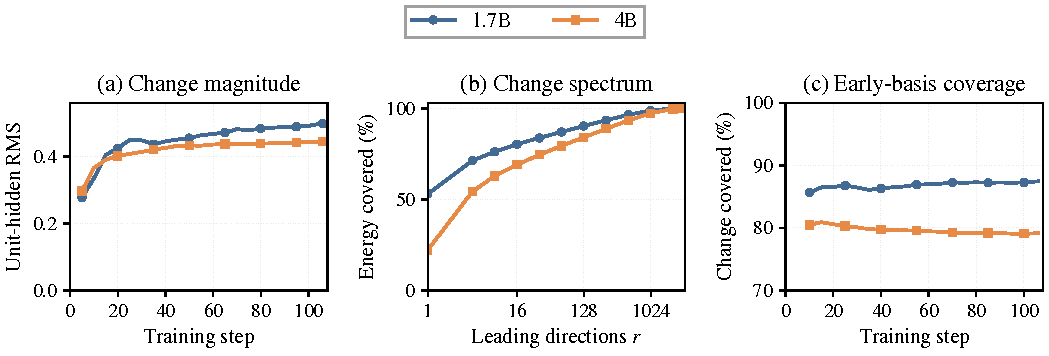
\includegraphics[width=\textwidth]{figures/rq2_adaptation.pdf}
\caption{Accumulated representation changes in paired FULL. (a) RMS change in unit-normalized hidden states from initialization, evaluated on fixed probe prefixes. (b) Cumulative representation change energy covered by the final checkpoint's own leading directions at step 106. The rank axis is logarithmic. (c) Coverage of cumulative representation change by the fixed step-10 rank-128 basis $U_{10}$. Markers identify the models. Lines connect recorded observations.}
\label{fig:rq2_adaptation}
\end{figure*}

\subsection{Representation-Space Gradient Dynamics}
\label{sec:rq2_gradients}
We next examine the supervision currently reaching the representation. With logits $z_t=W_th_t$, the individual-position hidden gradient is $g_{h,t}(c)=W_t^\top\nabla_{z_t}\ell_t(c)$.
Let $G_t$ contain these gradients as rows for the current sampled training responses, with $N_t$ positions and singular values $\sigma_{j,t}$. We summarize gradient strength by $\|G_t\|_F/\sqrt{N_t}$. To describe its distribution across directions, set $w_{j,t}=\sigma_{j,t}^2/\sum_k\sigma_{k,t}^2$ and compute
\begin{equation}
 H_t(r)=\sum_{j=1}^{r}w_{j,t},\qquad
 R_t=\exp\!\left(-\sum_jw_{j,t}\log w_{j,t}\right).
 \label{eq:rq2_gradient_spectrum}
\end{equation}
Here $H_t(r)$ is cumulative gradient-energy coverage and $R_t$ is energy effective rank.

The current signal weakens as its normalized energy distribution becomes more spread out (Figure~\ref{fig:rq2_gradients}). Between the first and final observations, gradient RMS decreases at both scales, while effective rank increases from 110.16 to 303.36 in 1.7B and from 87.41 to 371.55 in 4B (Table~\ref{tab:rq2_summary}). The intermediate measurements show fluctuations around this broad change. The final gradient spectra still have prominent leading directions, although these directions cover less energy than equally sized subspaces of representation change. 
\begin{figure*}[t]
\centering
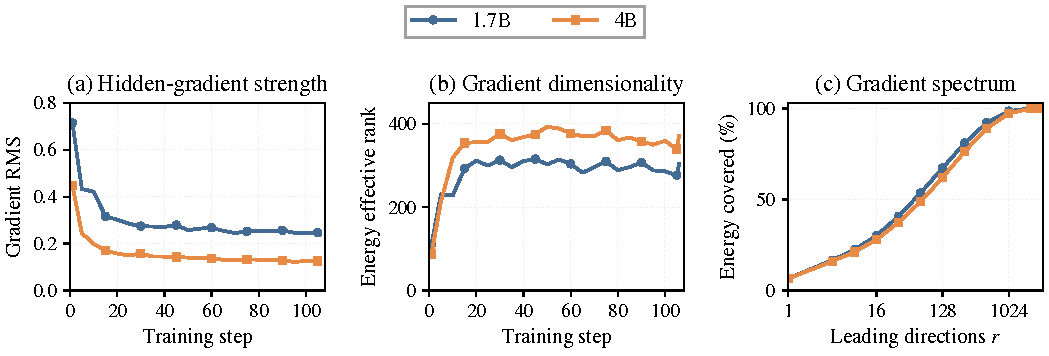
\includegraphics[width=\textwidth]{figures/rq2_gradient_dynamics.pdf}
\caption{Current hidden-gradient structure in paired FULL. (a) Per-position gradient RMS and (b) energy effective rank over training. (c) Cumulative gradient energy captured by the current gradient matrix's own leading directions at step 106. All panels use the full hidden space and sampled training responses. Lines connect measured observations. The spectrum uses a logarithmic rank axis.}
\label{fig:rq2_gradients}
\end{figure*}

\subsection{Gradient Coverage by Early Adaptation Directions}
\label{sec:rq2_coverage}
Although we have examined accumulated representation changes
and hidden-gradient dynamics separately, it remains unclear
whether the remaining gradient energy is concentrated along
the directions established during early representation adaptation.
To answer this question, we project the hidden gradients onto
the fixed early adaptation subspace $U_{10}$ and measure the
fraction of gradient energy it captures,
\begin{equation}
 A_t=\frac{\|G_tU_{10}\|_F^2}{\|G_t\|_F^2}.
 \label{eq:rq2_gradient_coverage}
\end{equation}
At the endpoint, $U_{10}$ covers 87.46\% and 79.16\% of accumulated representation change energy in 1.7B and 4B, respectively, and 16.71\% and 15.18\% of current gradient energy (Figure~\ref{fig:rq2_coverage}). Most current gradient energy therefore lies outside these early adaptation directions.

An equal-rank comparison clarifies the role of direction choice. The current gradients' own leading 128 directions capture 67.31\% and 62.12\% of their energy at the two scales, substantially exceeding coverage by $U_{10}$ (Table~\ref{tab:rq2_summary}). Current supervision retains concentrated directions, while the early adaptation basis provides limited coverage of those gradients. The comparisons use fixed probe prefixes for representation change and current sampled responses for gradients, with $U_{10}$ held identical across the two measurements. They establish how current sensitivity is distributed relative to historical adaptation. The effect of an executed update on unseen responses is examined in RQ3.

\begin{figure*}[t]
\centering
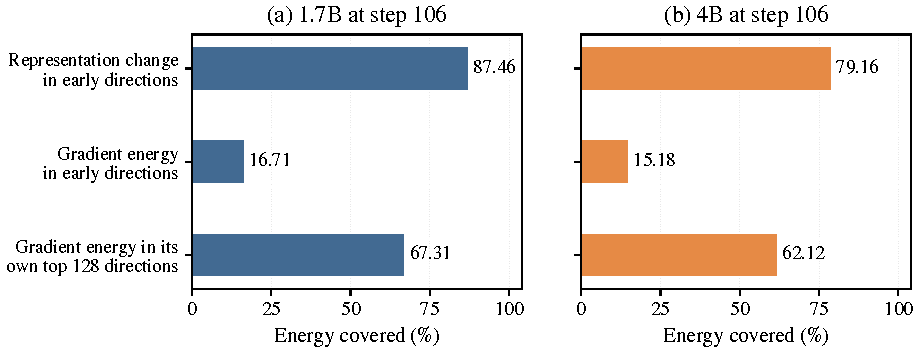
\includegraphics[width=0.85\textwidth]{figures/rq2_gradient_coverage.pdf}
\caption{Representation changes and hidden-gradient directions at the end step. We identify the top 128 directions of accumulated representation change at step 10 and keep them fixed. These early directions capture most of the accumulated representation change, but only a small fraction of the hidden-gradient energy at step 106. For comparison, the third bar shows the gradient energy captured by the gradient's own top 128 directions. Representation changes are measured on fixed probe prefixes, while gradients are measured on sampled training responses.}
\label{fig:rq2_coverage}
\end{figure*}

\begin{table}[t]
\centering
\caption{Core paired FULL representation results. Arrows give the first and last stated observations. Coverage entries are percentages. Full trajectories and spectra appear in Appendices~\ref{app:displacement} and~\ref{app:supplementary}.}
\label{tab:rq2_summary}
\footnotesize
\setlength{\tabcolsep}{2pt}
\begin{tabular}{lrr}
\toprule
Measurement & 1.7B & 4B \\
\midrule
\multicolumn{3}{l}{\textit{Representation change, step 10 $\to$ 106}}\\
Unit-hidden RMS & $.3350\to.4984$ & $.3657\to.4457$\\
Own-1 coverage & $38.81\to53.02$ & $22.90\to22.24$\\
Own-128 coverage & $85.66\to90.36$ & $80.50\to84.14$\\
Fixed-$U_{10}$ coverage & $85.66\to87.46$ & $80.50\to79.16$\\
\midrule
\multicolumn{3}{l}{\textit{Hidden gradients, step 1 $\to$ 106}}\\
RMS & $.7149\to.2397$ & $.4469\to.1238$\\
Energy effective rank & $110.16\to303.36$ & $87.41\to371.55$\\
Own-128 coverage & $74.12\to67.31$ & $75.52\to62.12$\\
Fixed-$U_{10}$ coverage (106) & 16.71 & 15.18\\
\bottomrule
\end{tabular}
\end{table}
\FloatBarrier

\begin{tcolorbox}[
    enhanced,
    breakable,
    colback=findingbg,
    colframe=findingblue,
    boxrule=0.7pt,
    arc=1.5mm,
    left=7pt,
    right=7pt,
    top=6pt,
    bottom=6pt,
    before skip=8pt,
    after skip=8pt
]
\textbf{\textcolor{findingblue}{Key Finding}}
The teacher calls for changes across a much broader set of representation directions than those that dominate the student's accumulated changes. As training progresses, these correction signals become weaker and more spread out, while a small set of early directions continues to explain most of the accumulated representation change.
\end{tcolorbox}


% RQ3

\section{RQ3}
\label{sec:RQ3}
\label{sec:generalization}

To examine how much OPD learning transfers to unseen
responses, we study three complementary aspects:
(1) \textbf{Validation Performance}, which tracks
how teacher KL and answer accuracy on held-out
questions evolve throughout training;
(2) \textbf{Transfer from Individual Updates}, which
measures the actual improvement produced by a single
training update on held-out responses, both in
magnitude and in the fraction of responses improved;
and (3) \textbf{Gradient Alignment Across Examples},
which examines how the directions of gradients from
training and validation examples, as well as different
training subsets, change during training.
We use the paired FULL trajectories at both scales,
with additional results and diagnostics reported in
Appendices~\ref{app:observations}
and~\ref{app:supplementary}.

\subsection{Validation Performance}
\label{sec:rq3_validation}
We first examine how performance on the excluded validation questions changes during training. At checkpoint $t$, the student generates a fresh response to each question. For a response $b$ containing $n_b$ positions, let $L_b(\theta)=n_b^{-1}\sum_i\ell_\theta(c_{bi})$. The validation loss averages these response losses, $K_V(\theta)=M^{-1}\sum_{b=1}^{M}L_b(\theta)$, where $M$ is the number of validation responses. Answer accuracy is the fraction of these responses with a correct final answer.

Validation KL decreases substantially at both scales, with the largest changes occurring early (Figure~\ref{fig:rq3_validation}a). Accuracy also improves early, followed by fluctuations over a narrower range (Figure~\ref{fig:rq3_validation}b). Table~\ref{tab:rq3_summary} summarizes the changes, and Table~\ref{tab:two_scale_validation} reports every observation. Continued agreement with the teacher therefore accompanies limited further improvement in sampled answer accuracy.

\begin{table}[t]
\centering
\caption{Validation performance and gradient alignment during
on-policy distillation. Validation metrics compare steps 10 and 106,
while single-update and gradient measurements compare steps 10 and 100.
Accuracy, relative KL improvement, and the fraction of improved
responses are reported as percentages.}
\label{tab:rq3_summary}
\footnotesize
\setlength{\tabcolsep}{2pt}
\begin{tabular}{lrr}
\toprule
Measurement & 1.7B & 4B \\
\midrule
Validation KL & $0.1742\!\to\!0.0784$ & $0.0976\!\to\!0.0445$\\
Validation accuracy & $7.03\!\to\!12.50$ & $25.78\!\to\!28.13$\\
Relative one-update gain & $7.20\!\to\!0.20$ & $6.53\!\to\!0.07$\\
Responses with lower KL & $100.00\!\to\!63.28$ & $98.44\!\to\!47.66$\\
Train--validation cosine & $0.913\!\to\!0.221$ & $0.922\!\to\!0.193$\\
Subset parameter cosine & $0.732\!\to\!0.083$ & $0.770\!\to\!0.060$\\
Subset hidden cosine & $0.898\!\to\!0.232$ & $0.889\!\to\!0.246$\\
Top-4 covariance overlap & $0.953\!\to\!0.890$ & $0.970\!\to\!0.947$\\
\bottomrule
\end{tabular}
\end{table}

\begin{figure*}[t]
\centering
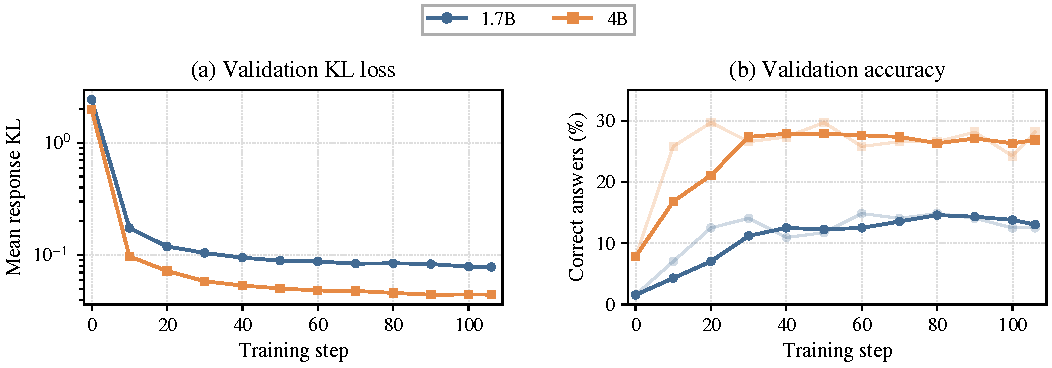
\includegraphics[width=\textwidth]{figures/rq3_validation.pdf}
\caption{Validation loss and answer accuracy over training.
At each checkpoint, the student generates new responses
to the same 128 held-out questions.
(a) Mean response KL on a logarithmic scale.
(b) Answer accuracy, with light lines showing individual
measurements and dark lines showing moving averages
over three observations.}
\label{fig:rq3_validation}
\end{figure*}

\subsection{Transfer from Individual Updates}
\label{sec:rq3_updates}

To measure the effect of individual training updates on
unseen responses, we evaluate validation KL loss before
and after the next actual AdamW update on a training batch.
At each checkpoint $t$, the student generates new responses
to held-out questions, which are kept fixed during the
before-and-after comparison.
Let $\theta_t^+=\theta_t+\Delta\theta_t$ denote the updated
parameters. We define the KL loss reduction for each
response and its average across validation responses as
\begin{equation}
 G_{b,t}=L_b(\theta_t)-L_b(\theta_t^+),\qquad
 G_{V,t}=\frac{1}{M}\sum_{b=1}^{M}G_{b,t}.
 \label{eq:rq3_gain}
\end{equation}
A positive $G_{b,t}$ indicates that the update reduces
the KL loss on response $b$.
We report the relative KL loss reduction
$G_{V,t}/K_V(\theta_t)$ and the fraction of responses
satisfying $G_{b,t}>10^{-6}$.
These metrics measure how much an update improves
validation responses and how many responses benefit.

The improvement from individual updates decreases
substantially over training
(Figure~\ref{fig:rq3_single_update}).
From checkpoint 10 to 100, the relative reduction
in validation KL loss drops from 7.20\% to 0.20\%
for 1.7B and from 6.53\% to 0.07\% for 4B
(Table~\ref{tab:rq3_summary}).
This decline persists after normalization by the
pre-update KL loss, indicating that each update
removes a smaller fraction of the remaining loss.
Some later updates even increase the mean validation
KL loss, despite its overall decrease throughout
training. Detailed results are reported in
Appendix~\ref{app:rq3_update_distribution}.

The fraction of responses benefiting from each update
also decreases. At checkpoint 10, nearly all validation
responses show lower KL loss after the update.
By checkpoint 100, this fraction falls to 63.28\%
for 1.7B and 47.66\% for 4B.
Notably, the 4B update still reduces the average
validation KL loss even though fewer than half of
the responses improve.
Thus, an average reduction in KL loss can mask
uneven improvements across unseen responses.
These measurements reflect changes in KL loss
on fixed responses rather than changes in
answer correctness.

\begin{figure*}[t]
\centering
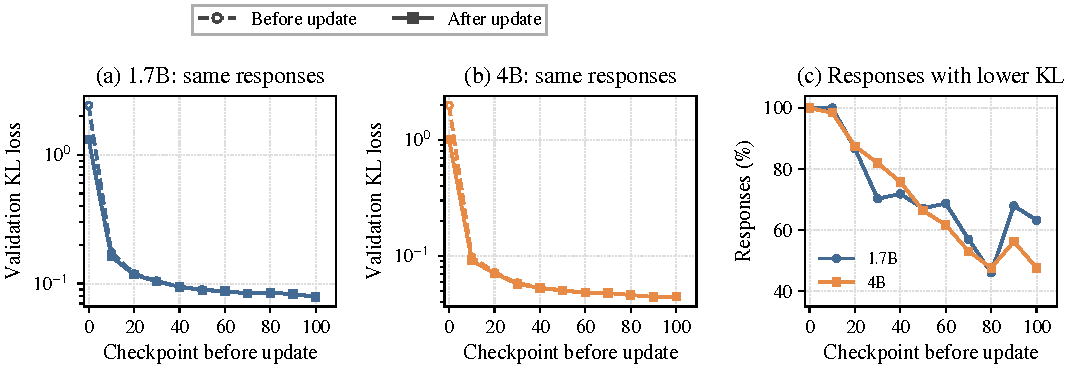
\includegraphics[width=\textwidth]{figures/rq3_single_update.pdf}
\caption{Effect of one actual training update on unseen responses. (a,b) Validation KL immediately before and after the update, evaluated on identical responses within each pair. Both axes for KL loss are logarithmic. The before/after curves approach each other as one-update improvements shrink. (c) Fraction of validation responses whose KL decreases by more than $10^{-6}$. The horizontal axis gives the checkpoint before the update; responses are freshly generated at each checkpoint and then fixed for its comparison.}
\label{fig:rq3_single_update}
\label{fig:two_scale_transfer}
\end{figure*}

\begin{figure*}[t]
\centering
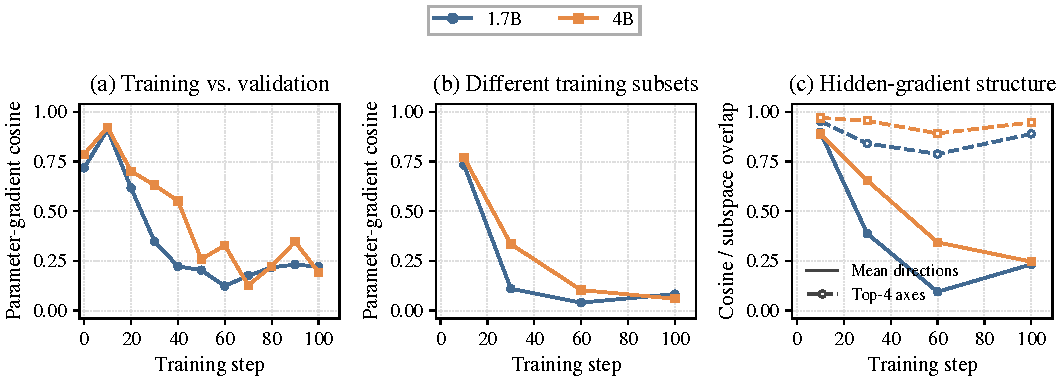
\includegraphics[width=\textwidth]{figures/rq3_gradient_agreement.pdf}
\caption{Gradient agreement during training. (a) Cosine between training and validation parameter gradients at the same checkpoint. (b) Mean parameter-gradient cosine across six pairs of four disjoint training subsets. (c) Mean cosine between subset-averaged hidden gradients and overlap of their top-4 centered covariance subspaces, using all hidden dimensions. Mean directions become less aligned while covariance axes remain similar. Lines connect the recorded observations.}
\label{fig:rq3_agreement}
\end{figure*}

\subsection{Gradient Alignment Across Examples}
\label{sec:rq3_agreement}

We next examine whether the declining benefit of
individual updates is accompanied by weaker gradient
alignment across examples.
Let $g_T$ be the training parameter gradient defined
in Section~\ref{sec:preliminaries and setup}, and
$g_V=\nabla_\theta K_V(\theta_t)$ the validation
parameter gradient at the same checkpoint.
We measure their alignment using cosine similarity:
\begin{equation}
 a_{TV,t}=\frac{g_T^\top g_V}{\|g_T\|_2\|g_V\|_2}.
 \label{eq:rq3_alignment}
\end{equation}
We also divide the training examples into four disjoint
subsets and compute their parameter gradients at the
same checkpoint. We report the average cosine similarity
across the six subset pairs to measure gradient alignment
among training examples.

Both measures of parameter-gradient alignment decrease
substantially during training
(Figure~\ref{fig:rq3_agreement}a,b;
Table~\ref{tab:rq3_summary}).
Late cross-subset cosine similarities are mostly small
and positive, with occasional negative values in 1.7B
(Table~\ref{tab:two_scale_batch}).
This decline accompanies the smaller transfer gains
observed in the preceding section.
However, weaker alignment does not necessarily imply
stronger conflict between examples: cosine similarity
can also decrease when mean gradients become small
relative to variation across examples.

To examine alignment at the representation level,
we also analyze gradients in the full hidden-state
space, as in RQ2.
For subset $b$, define the mean token gradient
$\mu_b=\mathbb E_b[g_h]$ and centered covariance
$\Sigma_b=\mathbb E_b[(g_h-\mu_b)(g_h-\mu_b)^\top]$.
We compare mean-gradient cosine similarities and
the overlap between leading covariance subspaces.
For top-$k$ eigenvector matrices $V_{a,k}$ and
$V_{b,k}$, subspace overlap is
$\|V_{a,k}^\top V_{b,k}\|_F^2/k$.

Mean hidden-gradient directions become less aligned,
while the leading covariance subspaces retain high
overlap at both scales
(Figure~\ref{fig:rq3_agreement}c).
The covariance subspaces describe the main directions
of gradient variation, whereas the mean gradients
indicate the average direction of the update signal
from each subset.
Thus, different subsets can share similar directions
of gradient variation even when their mean gradients
point in different directions.
Together, these results show that declining
single-update gains accompany weaker gradient
alignment across examples, despite the persistent
overlap in their covariance subspaces.
These observations do not establish a causal
relationship; identifying the cause of reduced
transfer requires controlling for gradient magnitude,
sampling variation, and the actual update direction.

\FloatBarrier
\begin{tcolorbox}[
 enhanced, breakable,
 colback=findingbg, colframe=findingblue,
 boxrule=0.7pt, arc=1.5mm,
 left=7pt, right=7pt, top=6pt, bottom=6pt,
 before skip=8pt, after skip=8pt
]
\textbf{\textcolor{findingblue}{Key Finding.}}
As OPD progresses, individual training updates
produce smaller reductions in KL loss on unseen
responses and improve fewer responses.
Meanwhile, gradients from different examples
become less aligned, although their dominant
directions of variation remain similar.
Validation KL loss continues to decrease,
while answer accuracy shows limited further
improvement in later training.
\end{tcolorbox}


% RQ4
\section{RQ4}
\label{sec:efficiency}

RQ2 showed that the leading directions of accumulated representation change become similar across successive checkpoints. This suggests a possible stopping rule. Once those directions stabilize, how much benchmark performance can the student retain if training ends there? We test this with \textbf{Adaptive early stop}. RQ3 motivates a second question. Even when the student generates fresh responses for every update, late updates produce only small KL improvements on unseen responses. Given the cost of generation and teacher scoring, how much does refreshing the batch at every update buy? We test this with \textbf{Rollout reuse}, keeping the number of updates fixed and refreshing the batch every other update.

\subsection{Adaptive early stop}
Every five updates, we evaluate the same probe prefixes and compute the leading $r=128$ eigenvectors $U_t$ of the representation-change matrix $C_t$ defined in Equation~\ref{eq:rq2_representation_change}. For checkpoints $i$ and $j$, let $s_k=\sigma_k^2(U_i^\top U_j)$ for $k=1,\ldots,r$. Their mean $O_{ij}=r^{-1}\sum_k s_k$ measures subspace overlap, and their tenth percentile $Q_{ij}$ checks whether the overlap extends to the less aligned directions. We also measure the fraction of change energy at step $t$ captured by a basis $U$ as $E_t(U)=\operatorname{tr}(U^\top C_t U)/\operatorname{tr}(C_t)$.

At each check $t\geq15$, let $a=t-10$ and $b=t-5$. We stop at the first check for which all four conditions hold:
\begin{equation}
\begin{aligned}
 \min(O_{ab},O_{bt}) &\geq 0.98,\\
 O_{at} &\geq 0.97,\\
 \min(Q_{ab},Q_{bt},Q_{at}) &\geq 0.90,\\
 [E_t(U_t)-E_t(U_a)]_+ &\leq 0.005 .
\end{aligned}
\label{eq:rq4_stop}
\end{equation}
Here $[x]_+=\max(x,0)$. The adjacent and endpoint checks require stability throughout the three-checkpoint window. The last condition requires the earliest basis in the window to capture the latest representation changes to within half a percentage point of the current basis.

The rule first triggered at update 40 for 1.7B and update 50 for 4B, compared with 106 updates in FULL. Stopping at those checkpoints saved 65.0\% and 48.1\% of total training time. The five-benchmark average decreased by 0.40 and 0.38 percentage points, respectively (Table~\ref{tab:benchmark_summary}).

\subsection{Rollout reuse}
FULL generates a batch of responses, queries the teacher, and takes one optimizer step. Rollout reuse takes a second step on the same responses and cached teacher targets. Before that second step, we recompute the student predictions and gradients at the updated parameters. Both runs take 106 optimizer steps, so the comparison tests the cost of reducing fresh rollout rounds from 106 to 53.

The second update reduced KL on the cached responses at all 11 measured checkpoints in each model. The saved generation and teacher work translated into a 44.8\% reduction in total training time for 1.7B and a 35.0\% reduction for 4B. The corresponding benchmark averages fell by 0.29 and 0.96 percentage points (Table~\ref{tab:benchmark_summary}). Thus, both students could fit the cached responses further, while the larger student incurred a greater benchmark cost from refreshing the training data less often.

\begin{table*}[t]
\centering
\caption{Training cost and final performance. Rounds count fresh rollout batches. Time covers the full training run, and savings are relative to FULL at the same model size. Task scores are Mean@8 (\%), and Avg.\ is their arithmetic mean. Each trained configuration was run once.}
\label{tab:benchmark_summary}
\scriptsize
\setlength{\tabcolsep}{2.8pt}
\begin{tabular}{@{}llrrrrrrrrrr@{}}
\toprule
Model & Method & Rounds & Updates & Min. & Time saved & MATH500 & HMMT25 & HMMT26 & AIME26 & Minerva & Avg.\\
\midrule
\multirow{4}{*}{1.7B}
 & Base                & 0 & 0 & -- & -- & 13.35 & 0.00 & 0.76 & 0.00 & 3.72 & 3.57\\
 & FULL                & 106 & 106 & 214.8 & -- & 65.53 & 1.25 & 3.41 & 8.33 & 26.79 & 21.06\\
 & Adaptive early stop & 40 & 40 & 75.2 & 65.0\% & 65.60 & 1.67 & 4.92 & 4.58 & 26.52 & 20.66\\
 & Rollout reuse       & 53 & 106 & 118.6 & 44.8\% & 66.48 & 1.25 & 3.41 & 6.67 & 26.06 & 20.77\\
\midrule
\multirow{4}{*}{4B}
 & Base                & 0 & 0 & -- & -- & 23.12 & 0.00 & 1.14 & 1.25 & 9.88 & 7.08\\
 & FULL                & 106 & 106 & 234.6 & -- & 80.28 & 6.67 & 12.12 & 12.92 & 39.94 & 30.38\\
 & Adaptive early stop & 50 & 50 & 121.6 & 48.1\% & 79.58 & 7.92 & 9.09 & 14.17 & 39.25 & 30.00\\
 & Rollout reuse       & 53 & 106 & 152.5 & 35.0\% & 78.60 & 8.33 & 8.71 & 13.33 & 38.10 & 29.42\\
\bottomrule
\end{tabular}
\end{table*}
\FloatBarrier



\FloatBarrier
\section{Discussion and Conclusion}

\input{sections/discussion}

\input{sections/conclusion}

\section*{Impact Statement}
This work studies the dynamics and computational costs of language-model distillation. More efficient training can reduce resource use and lower barriers to model adaptation, while also making capable models easier to deploy. Our mathematical-reasoning evaluations do not establish safety or reliability in other applications; deployment requires evaluation appropriate to the intended use.

\bibliography{example_paper}
\bibliographystyle{icml2025}


%%%%%%%%%%%%%%%%%%%%%%%%%%%%%%%%%%%%%%%%%%%%%%%%%%%%%%%%%%%%%%%%%%%%%%%%%%%%%%%
%%%%%%%%%%%%%%%%%%%%%%%%%%%%%%%%%%%%%%%%%%%%%%%%%%%%%%%%%%%%%%%%%%%%%%%%%%%%%%%
% APPENDIX
%%%%%%%%%%%%%%%%%%%%%%%%%%%%%%%%%%%%%%%%%%%%%%%%%%%%%%%%%%%%%%%%%%%%%%%%%%%%%%%
%%%%%%%%%%%%%%%%%%%%%%%%%%%%%%%%%%%%%%%%%%%%%%%%%%%%%%%%%%%%%%%%%%%%%%%%%%%%%%%
\clearpage
\appendix
\onecolumn
\begin{center}
{\Large\scshape Appendix}\\[7pt]
{\large\papertitle}
\end{center}
\setcounter{figure}{0}
\setcounter{table}{0}
\counterwithin{figure}{section}
\counterwithin{table}{section}
\section{Experimental Settings}
\label{app:settings}
Table~\ref{tab:settings} specifies the original two-scale study. Tables~\ref{tab:paired_settings} and~\ref{tab:paired4b_settings} specify the paired FULL/Adapter studies. Each paired branch follows its own sampled training trajectory under the same protocol. All reported distillation experiments use the selected-support objective in Equation~\ref{eq:loss}; model-size comparisons jointly vary student and teacher capacity.

\begin{table}[!htbp]
\centering
\caption{Experimental settings. Each student is distilled from the post-trained Qwen3 model of the same size. Training uses one sampled response per prompt; benchmark evaluation uses independent repeated samples.}
\label{tab:settings}
\small
\setlength{\tabcolsep}{3pt}
\begin{tabular}{lll}
\toprule
Setting & 1.7B & 4B \\
\midrule
Student & Qwen3-1.7B-Base & Qwen3-4B-Base \\
Teacher & Qwen3-1.7B & Qwen3-4B \\
Training set & Filtered DAPO14k & Filtered DAPO14k \\
Training prompts & 13,534 & 13,534 \\
Hidden dim. / probe positions & 2,048 / 5,514 & 2,560 / 6,146 \\
Generated / optimized responses & 160 / 128 & 160 / 128 \\
Optimizer & AdamW & AdamW \\
Learning rate / schedule & $10^{-5}$ / constant & $10^{-5}$ / constant \\
$\beta_1,\beta_2$ / weight decay & (0.9, 0.999) / 0.01 & (0.9, 0.999) / 0.01 \\
Gradient clipping / warmup & 1.0 / none & 1.0 / none \\
Max. prompt / training response & 1,024 / 2,048 & 1,024 / 2,048 \\
Sampling temperature / top-p & 1.0 / 1.0 & 1.0 / 1.0 \\
Benchmark samples / max. response & 8 / 8,192 & 8 / 8,192 \\
Evaluation seed & 42 & 42 \\
Benchmark scoring & Original grader & Lenient answer grader \\
Observation basis rank / step & 128 / 10 & 128 / 10 \\
\bottomrule
\end{tabular}
\end{table}

\begin{table}[!htbp]
\centering
\caption{Additional protocol for the paired 1.7B study. Both branches use the same student--teacher pair and Top-16 objective as the original study. The fixed validation questions are excluded from the training pool. The Adapter branch learns its basis within its own warmup.}
\label{tab:paired_settings}
\small
\setlength{\tabcolsep}{3pt}
\begin{tabular}{ll}
\toprule
Paired-study setting & Value \\
\midrule
Train / validation questions & 128 / 128 \\
Updates / reuse / GPUs / microbatch & 106 / 1 / 2 / 4 \\
Validation interval / terminal step & 10 / 106 \\
Cross-batch checkpoints & 10, 30, 60, 100 \\
Disjoint batches / questions each & 4 / 32 \\
Repeated-rollout steps & 10, 50, 100 \\
Questions / rollouts per question & 4 / 4 \\
Adapter rank / hidden dimension & 128 / 2,048 \\
Stability interval / minimum step & 5 / 15 \\
Window / adjacent / endpoint & 3 / 0.98 / 0.97 \\
Decile $\cos^2$ / energy-gap limit & 0.90 / 0.005 \\
Switch step / Adapter updates & 40 / 66 \\
Adapter LR / warmup updates & $10^{-5}$ / 10 \\
Guard tokens per GPU / backtracks & 128 / 6 \\
Mean / max. policy-KL limit & 0.002 / 0.02 \\
Hidden / relative teacher-KL limit & 0.01 / 0.05 \\
Benchmark scoring / samples & Lenient answer / 8 \\
\bottomrule
\end{tabular}
\end{table}

\begin{table}[!htbp]
\centering
\caption{4B. Additional protocol for the paired 4B study. Both branches use the same student--teacher pair and Top-16 objective as the original study. The fixed validation questions are excluded from the training pool. The Adapter branch learns its basis within its own warmup.}
\label{tab:paired4b_settings}
\small
\setlength{\tabcolsep}{3pt}
\begin{tabular}{ll}
\toprule
Paired-study setting & Value \\
\midrule
Train / validation questions & 128 / 128 \\
Updates / reuse / GPUs / microbatch & 106 / 1 / 2 / 4 \\
Validation interval / terminal step & 10 / 106 \\
Cross-batch checkpoints & 10, 30, 60, 100 \\
Disjoint batches / questions each & 4 / 32 \\
Repeated-rollout steps & 10, 50, 100 \\
Questions / rollouts per question & 4 / 4 \\
Adapter rank / hidden dimension & 128 / 2,560 \\
Stability interval / minimum step & 5 / 15 \\
Window / adjacent / endpoint & 3 / 0.98 / 0.97 \\
Decile $\cos^2$ / energy-gap limit & 0.90 / 0.005 \\
Switch step / Adapter updates & 50 / 56 \\
Adapter LR / warmup updates & $10^{-5}$ / 10 \\
Guard tokens per GPU / backtracks & 128 / 6 \\
Mean / max. policy-KL limit & 0.002 / 0.02 \\
Hidden / relative teacher-KL limit & 0.01 / 0.05 \\
Benchmark scoring / samples & Lenient answer / 8 \\
\bottomrule
\end{tabular}
\end{table}


\FloatBarrier
\section{Supplementary Token-Score Diagnostics}
\label{app:token_scores}
We compare token scores as supplementary diagnostics at the final 1.7B and 4B checkpoints (Tables~\ref{tab:paired_selectors} and~\ref{tab:paired4b_selectors}). Each score selects the same fraction of positions. The tables report captured KL and hidden-gradient energy; these scores do not alter the recorded training updates.

\paragraph{Disagreement, uncertainty, and log-ratio variance.}
All scores use the conditional distributions in Equation~\ref{eq:loss}. We record KL, total variation $\frac12\sum_v|\tilde p_v-\tilde q_v|$, and student entropy $H=-\sum_v\tilde p_v\log\tilde p_v$. For $r_v=\log(\tilde p_v/\tilde q_v)$, the log-ratio variance is $V=\operatorname{Var}_{\tilde p}(r_v)$. This variance appears as the reverse-KL local utility in \citet{sadagopan2026utility} and as the Fisher-metric signal term in \citet{sheng2026ier}.

\paragraph{TIP-inspired entropy--KL combination.}
Following the Soft-OR construction of \citet{xu2026tip}, we compute $s=\bar H+\bar K-\bar H\bar K$, where bars denote batchwise min--max normalization. Our measurements apply this score to the recorded Top-16 conditional distributions. They evaluate the score under our checkpoint protocol; the paper's complete token-selection training procedure is outside this comparison.

\paragraph{Information-efficiency ratio.}
Following \citet{sheng2026ier}, we evaluate the conditional-support information-efficiency ratio (IER)
\begin{equation}
 b=\frac{\sum_v(1-\tilde p_v)r_v}{\sum_v(1-\tilde p_v)},\qquad
 \operatorname{IER}=\frac{V}{\sum_v(1-\tilde p_v)(r_v-b)^2-V}.
\end{equation}
We rank valid positive-denominator cases. IER concerns a sampled next-token gradient estimator; our training directly evaluates the selected-support loss. Thus, the table measures a hypothetical estimator's reliability under the cached conditional distributions.

\paragraph{Representation-dependent diagnostics.}
We additionally define retention $\rho=\|U^\top g_h\|^2/\|g_h\|^2$ and the combined score $s\rho$ to inspect the measured subspace. These are geometric diagnostics used in this study. At both scales, disagreement and log-ratio variance capture more full-hidden gradient energy than entropy; retention alone captures little total energy, while the combination shifts selection toward projected energy. A training intervention would be needed to establish benefits from using these rankings during optimization.

\begin{table*}[!htbp]
\centering
\caption{Signal captured by the highest-scoring decile at the final paired-study checkpoint. Each cell reports FULL. Columns give captured KL, full hidden-gradient energy, and $U$-projected energy, all in percent. Scores are observational diagnostics.}
\label{tab:paired_selectors}
\small
\setlength{\tabcolsep}{3pt}
\begin{tabular}{lrrr}
\toprule
Selection score & KL & Full energy & $U$ energy \\
\midrule
KL & 77.06 & 84.69 & 84.36 \\
Total variation & 74.37 & 78.81 & 77.83 \\
Entropy & 37.37 & 38.29 & 29.04 \\
Entropy--KL mixture & 40.68 & 42.71 & 34.76 \\
Log-ratio variance & 71.91 & 86.78 & 86.33 \\
Estimator reliability & 59.17 & 80.25 & 76.53 \\
$U$ retention & 11.70 & 7.56 & 21.17 \\
Mixture $\times$ retention & 37.65 & 38.62 & 63.92 \\
\bottomrule
\end{tabular}
\end{table*}

\begin{table*}[!htbp]
\centering
\caption{4B. Signal captured by the highest-scoring decile at the final paired-study checkpoint. Each cell reports FULL. Columns give captured KL, full hidden-gradient energy, and $U$-projected energy, all in percent. Scores are observational diagnostics.}
\label{tab:paired4b_selectors}
\small
\setlength{\tabcolsep}{3pt}
\begin{tabular}{lrrr}
\toprule
Selection score & KL & Full energy & $U$ energy \\
\midrule
KL & 74.79 & 81.87 & 79.06 \\
Total variation & 72.49 & 79.71 & 77.50 \\
Entropy & 39.22 & 40.04 & 31.85 \\
Entropy--KL mixture & 43.47 & 44.46 & 37.04 \\
Log-ratio variance & 70.11 & 83.34 & 80.63 \\
Estimator reliability & 59.99 & 76.14 & 70.79 \\
$U$ retention & 6.66 & 5.23 & 16.22 \\
Mixture $\times$ retention & 32.37 & 32.84 & 61.36 \\
\bottomrule
\end{tabular}
\end{table*}


\FloatBarrier
\section{Displacement and Basis Discovery}
\label{app:displacement}
Figure~\ref{fig:rq2_adaptation} uses the paired FULL trajectories, matching the main supervision and gradient analyses. Tables~\ref{tab:paired_adapter_geometry} and~\ref{tab:paired4b_adapter_geometry} provide their endpoint values. The separate original studies replicate the displacement/gradient coverage contrast and show strong overlap between nearby late-checkpoint bases (Table~\ref{tab:subspace}). For rank-$r$ orthonormal bases, overlap is $\|U_a^\top U_b\|_F^2/r$.




\begin{table}[t]
\centering
\caption{Geometry at the final FULL checkpoint. Own-$r$ rows give cumulative displacement energy captured by that checkpoint\textquotesingle s leading directions. Fixed-$U$ uses the step-10 basis. The last two rows measure subspace overlap. All entries are percentages.}
\label{tab:subspace}
\small
\setlength{\tabcolsep}{3pt}
\begin{tabular}{lrr}
\toprule
Metric (\%) & 1.7B & 4B \\
\midrule
Own-1 motion & 49.58 & 23.97 \\
Own-4 motion & 72.03 & 55.70 \\
Own-8 motion & 76.56 & 63.94 \\
Own-16 motion & 80.68 & 70.20 \\
Own-128 motion & 90.55 & 84.88 \\
Fixed-$U$ motion & 88.01 & 80.10 \\
Fixed-$U$ gradient & 16.79 & 15.18 \\
$U_{10},U_{106}$ overlap & 77.86 & 72.17 \\
$U_{100},U_{106}$ overlap & 99.46 & 98.72 \\
\bottomrule
\end{tabular}
\end{table}

\begin{table*}[!htbp]
\centering
\caption{1.7B paired FULL final displacement and gradient geometry. Own-$r$ coverage uses final displacement eigenvectors; fixed-$U$ uses the step-10 basis. Energy shares are percentages.}
\label{tab:paired_adapter_geometry}
\small
\setlength{\tabcolsep}{3pt}
\begin{tabular}{lr}
\toprule
Measurement & Value \\
\midrule
FULL final own-1 / own-128 & 53.02 / 90.36 \\
FULL final fixed-$U$ coverage & 87.46 \\
FULL final fixed-$U$ gradient energy & 16.71 \\
Hidden dimension / isotropic rank-128 share (\%) & 2048 / 6.25 \\
\bottomrule
\end{tabular}
\end{table*}

\begin{table*}[!htbp]
\centering
\caption{4B paired FULL final displacement and gradient geometry. Own-$r$ coverage uses final displacement eigenvectors; fixed-$U$ uses the step-10 basis. Energy shares are percentages.}
\label{tab:paired4b_adapter_geometry}
\small
\setlength{\tabcolsep}{3pt}
\begin{tabular}{lr}
\toprule
Measurement & Value \\
\midrule
FULL final own-1 / own-128 & 22.24 / 84.14 \\
FULL final fixed-$U$ coverage & 79.16 \\
FULL final fixed-$U$ gradient energy & 15.18 \\
Hidden dimension / isotropic rank-128 share (\%) & 2560 / 5.00 \\
\bottomrule
\end{tabular}
\end{table*}


\begin{table}[t]
\centering
\caption{First accepted stopping window. Checks occur every five updates, using three observations and starting no earlier than update 15. Overlaps and energy gap are percentages. Required minima: adjacent overlap 98\%, endpoints 97\%, lower-decile squared principal-angle cosine 90\%; maximum energy gap: 0.5 percentage points.}
\label{tab:stopping}
\small
\setlength{\tabcolsep}{3pt}
\begin{tabular}{lrr}
\toprule
Criterion & 1.7B & 4B \\
\midrule
Stop update & 40 & 50 \\
Adjacent min. (\%) & 98.70 & 98.43 \\
Endpoints (\%) & 97.96 & 97.40 \\
Lower decile (\%) & 96.21 & 95.49 \\
Energy gap (pp) & 0.13 & 0.14 \\
\bottomrule
\end{tabular}
\end{table}


\FloatBarrier
\subsection{Cumulative Displacement Magnitudes and Early-Basis Coverage}
\label{app:cumulative_magnitudes}
Table~\ref{tab:cumulative_motion_audit} reports every paired FULL motion observation from basis discovery onward. The fixed panels contain 5,203 positions for 1.7B and 6,481 for 4B. Both cumulative displacement magnitudes and early-basis coverage are retained, so the coverage percentages can be read alongside the absolute scale of the measured change.

\begin{table}[!htbp]
\centering
\caption{Cumulative displacement magnitude and fixed early-basis coverage at every recorded checkpoint from step 10 in paired FULL. RMS is the square root of the mean squared vector norm across fixed probe positions. Raw RMS uses unnormalized hidden states; unit RMS uses unit-normalized states. Coverage is measured on the unit-normalized displacement relative to initialization, using the fixed step-10 rank-128 basis. All entries describe cumulative changes.}
\label{tab:cumulative_motion_audit}
\small\setlength{\tabcolsep}{8pt}
\begin{tabular}{rrrrrrr}
\toprule
 & \multicolumn{3}{c}{1.7B} & \multicolumn{3}{c}{4B} \\
\cmidrule(lr){2-4}\cmidrule(lr){5-7}
Step & Raw RMS & Unit RMS & $U$ coverage (\%) & Raw RMS & Unit RMS & $U$ coverage (\%) \\
\midrule
10 & 47.357 & 0.33499 & 85.66 & 57.784 & 0.36566 & 80.50 \\
15 & 56.045 & 0.40512 & 86.50 & 62.306 & 0.39057 & 80.92 \\
20 & 58.821 & 0.42436 & 86.57 & 63.665 & 0.40182 & 80.59 \\
25 & 62.165 & 0.44992 & 86.79 & 64.463 & 0.40821 & 80.29 \\
30 & 61.876 & 0.44841 & 86.48 & 65.053 & 0.41356 & 80.09 \\
35 & 60.366 & 0.43684 & 86.10 & 65.947 & 0.42071 & 79.80 \\
40 & 61.393 & 0.44512 & 86.32 & 66.744 & 0.42587 & 79.72 \\
45 & 62.098 & 0.45074 & 86.51 & 67.666 & 0.43196 & 79.61 \\
50 & 62.610 & 0.45513 & 86.64 & 67.905 & 0.43286 & 79.62 \\
55 & 63.720 & 0.46361 & 86.92 & 67.924 & 0.43262 & 79.59 \\
60 & 64.293 & 0.46756 & 87.00 & 68.456 & 0.43603 & 79.46 \\
65 & 64.854 & 0.47148 & 87.08 & 68.694 & 0.43763 & 79.39 \\
70 & 66.268 & 0.48192 & 87.29 & 68.937 & 0.43856 & 79.27 \\
75 & 65.890 & 0.47819 & 87.24 & 68.876 & 0.43779 & 79.21 \\
80 & 66.648 & 0.48370 & 87.30 & 69.016 & 0.43847 & 79.24 \\
85 & 67.046 & 0.48624 & 87.24 & 69.241 & 0.43977 & 79.18 \\
90 & 67.386 & 0.48835 & 87.27 & 69.404 & 0.44056 & 79.19 \\
95 & 67.485 & 0.48898 & 87.24 & 69.804 & 0.44260 & 79.08 \\
100 & 67.865 & 0.49170 & 87.28 & 69.852 & 0.44290 & 79.06 \\
105 & 68.632 & 0.49771 & 87.44 & 70.200 & 0.44534 & 79.14 \\
106 & 68.707 & 0.49835 & 87.46 & 70.269 & 0.44572 & 79.16 \\
\bottomrule
\end{tabular}
\end{table}


\FloatBarrier
\section{Detailed FULL Observations}
\label{app:observations}
This appendix reports FULL validation histories, one-update measurements, and gradient geometry in both model sizes.

\begin{figure}[!htbp]
\centering
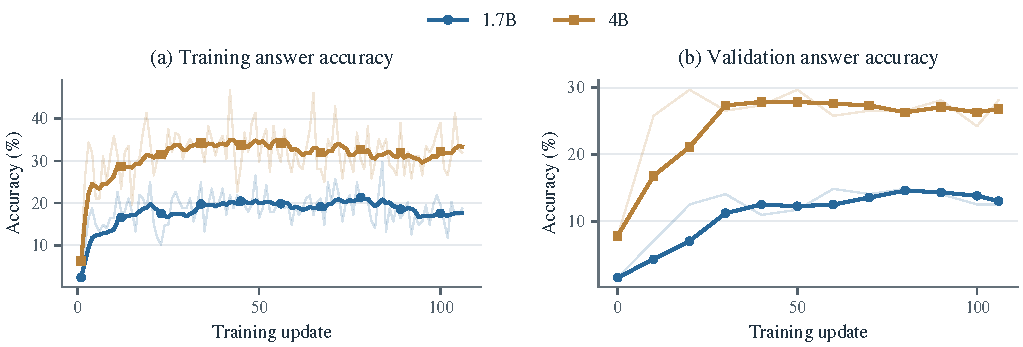
\includegraphics[width=\textwidth]{figures/accuracy_history.pdf}
\caption{FULL training and validation answer accuracy at both scales. Light curves retain raw observations; dark curves use trailing windows of ten updates for training and three observations for validation. Training responses are scored before optimization. Validation responses are freshly generated on the same excluded questions at each observation.}
\label{fig:accuracy_history}
\end{figure}
\begin{table}[!htbp]
\centering
\caption{Freshly generated answers on 128 validation questions excluded from training at each scale. Entries report FULL. Accuracy is percent; KL averages per-response token-mean losses.}
\label{tab:two_scale_validation}
\small
\setlength{\tabcolsep}{3pt}
\begin{tabular}{rrrrr}
\toprule
Step & 1.7B KL & 1.7B accuracy & 4B KL & 4B accuracy \\
\midrule
0 & 2.41500 & 1.56 & 1.97164 & 7.81 \\
10 & 0.17422 & 7.03 & 0.09756 & 25.78 \\
20 & 0.11939 & 12.50 & 0.07225 & 29.69 \\
30 & 0.10461 & 14.06 & 0.05850 & 26.56 \\
40 & 0.09494 & 10.94 & 0.05360 & 27.34 \\
50 & 0.08926 & 11.72 & 0.05054 & 29.69 \\
60 & 0.08781 & 14.84 & 0.04840 & 25.78 \\
70 & 0.08389 & 14.06 & 0.04799 & 26.56 \\
80 & 0.08461 & 14.84 & 0.04613 & 26.56 \\
90 & 0.08332 & 14.06 & 0.04441 & 28.13 \\
100 & 0.07893 & 12.50 & 0.04462 & 24.22 \\
106 & 0.07841 & 12.50 & 0.04450 & 28.13 \\
\bottomrule
\end{tabular}
\end{table}

\begin{table}[!htbp]
\centering
\caption{One-step validation transfer in paired-study FULL. Before/after losses use identical freshly generated validation prefixes. Actual and linear-predicted gains are multiplied by $10^3$; positive fraction uses gain $>10^{-6}$. Relative gain is $100G_V/(K_V(\theta)+10^{-12})$, with $K_V(\theta)$ evaluated on the same prefixes before the update. $c_g$ compares training and validation gradients.}
\label{tab:paired_transfer}
\small
\setlength{\tabcolsep}{3pt}
\begin{tabular}{lrrrrr}
\toprule
Before step  &  Actual  &  Predicted  &  Relative (\%)  &  Positive (\%)  &  $c_g$  \\
\midrule
0  &  1104.3261  &  9547.2064  &  45.735  &  100.00  &  0.7182  \\
10  &  12.5471  &  20.6128  &  7.202  &  100.00  &  0.9127  \\
20  &  2.2858  &  4.3104  &  1.915  &  86.72  &  0.6172  \\
30  &  0.7939  &  1.3757  &  0.759  &  70.31  &  0.3485  \\
40  &  0.5942  &  0.8148  &  0.626  &  71.88  &  0.2226  \\
50  &  0.4722  &  0.6193  &  0.529  &  67.19  &  0.2033  \\
60  &  0.4295  &  0.5707  &  0.489  &  68.75  &  0.1232  \\
70  &  0.2031  &  0.3146  &  0.242  &  57.03  &  0.1758  \\
80  &  -0.1346  &  0.1726  &  -0.159  &  46.09  &  0.2169  \\
90  &  0.5068  &  0.6088  &  0.608  &  67.97  &  0.2316  \\
100  &  0.1613  &  0.4004  &  0.204  &  63.28  &  0.2211  \\
\bottomrule
\end{tabular}
\end{table}

\begin{table}[!htbp]
\centering
\caption{4B. One-step validation transfer in paired-study FULL. Before/after losses use identical freshly generated validation prefixes. Actual and linear-predicted gains are multiplied by $10^3$; positive fraction uses gain $>10^{-6}$. Relative gain is $100G_V/(K_V(\theta)+10^{-12})$, with $K_V(\theta)$ evaluated on the same prefixes before the update. $c_g$ compares training and validation gradients.}
\label{tab:paired4b_transfer}
\small
\setlength{\tabcolsep}{3pt}
\begin{tabular}{lrrrrr}
\toprule
Before step  &  Actual  &  Predicted  &  Relative (\%)  &  Positive (\%)  &  $c_g$  \\
\midrule
0  &  966.1828  &  15190.3290  &  49.004  &  100.00  &  0.7868  \\
10  &  6.3733  &  12.3741  &  6.533  &  98.44  &  0.9220  \\
20  &  1.2939  &  2.3732  &  1.791  &  87.50  &  0.7011  \\
30  &  0.9536  &  1.6808  &  1.630  &  82.03  &  0.6321  \\
40  &  0.5023  &  0.8043  &  0.937  &  75.78  &  0.5518  \\
50  &  0.2109  &  0.4383  &  0.417  &  66.41  &  0.2588  \\
60  &  0.1734  &  0.3961  &  0.358  &  61.72  &  0.3278  \\
70  &  -0.0491  &  0.2486  &  -0.102  &  53.13  &  0.1267  \\
80  &  -0.0360  &  0.2738  &  -0.078  &  47.66  &  0.2230  \\
90  &  0.0017  &  0.3096  &  0.004  &  56.25  &  0.3463  \\
100  &  0.0319  &  0.2680  &  0.072  &  47.66  &  0.1927  \\
\bottomrule
\end{tabular}
\end{table}

\begin{figure}[!htbp]
\centering
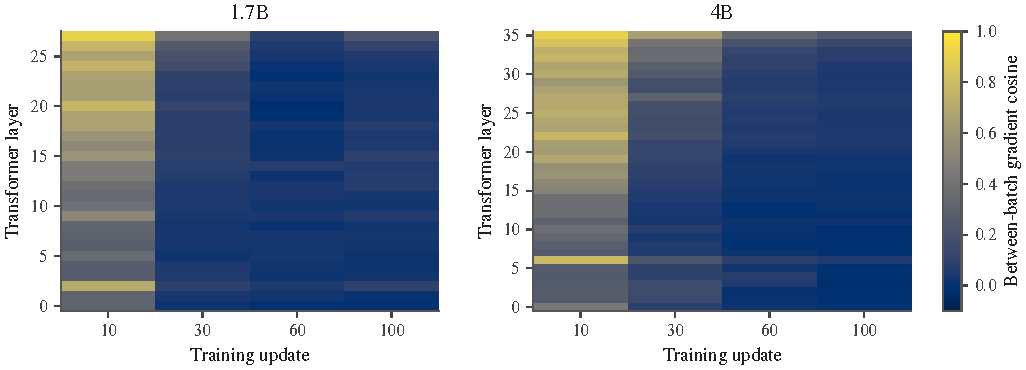
\includegraphics[width=\textwidth]{figures/two_scale_layers.pdf}
\caption{Layer-resolved FULL parameter-gradient agreement in both scales. Each heatmap compares four disjoint subsets at a fixed checkpoint; color is mean pairwise gradient cosine.}
\label{fig:two_scale_layers}
\end{figure}

\begin{table}[!htbp]
\centering
\caption{Adjacent-observation full-hidden gradient comparisons at both scales. Mean cosine retains signs; axis overlap is sign-invariant. Checkpoint and sampled batch both change across observations.}
\label{tab:two_scale_temporal}
\small
\setlength{\tabcolsep}{3pt}
\begin{tabular}{llrrrr}
\toprule
Model & Steps & Mean cosine & Axis-1 & Axes-4 & Axes-128 \\
\midrule
1.7B & 10--15 & -0.5526 & 0.9284 & 0.7837 & 0.7361 \\
1.7B & 15--20 & 0.1285 & 0.9840 & 0.9817 & 0.7701 \\
1.7B & 20--25 & -0.3374 & 0.9843 & 0.9809 & 0.7543 \\
1.7B & 25--30 & -0.2571 & 0.9680 & 0.8327 & 0.7536 \\
1.7B & 30--35 & -0.4686 & 0.9595 & 0.9857 & 0.7642 \\
1.7B & 35--40 & -0.1571 & 0.9887 & 0.9824 & 0.7592 \\
1.7B & 40--45 & -0.2392 & 0.9921 & 0.9543 & 0.7418 \\
1.7B & 45--50 & -0.1321 & 0.9890 & 0.9648 & 0.7452 \\
1.7B & 50--55 & -0.1673 & 0.9792 & 0.9630 & 0.7499 \\
1.7B & 55--60 & -0.0947 & 0.9797 & 0.9714 & 0.7305 \\
1.7B & 60--65 & -0.0592 & 0.9853 & 0.9829 & 0.7506 \\
1.7B & 65--70 & 0.0916 & 0.9837 & 0.9791 & 0.7667 \\
1.7B & 70--75 & 0.3569 & 0.9882 & 0.9862 & 0.7492 \\
1.7B & 75--80 & -0.1038 & 0.9894 & 0.9760 & 0.7448 \\
1.7B & 80--85 & -0.2730 & 0.9874 & 0.9737 & 0.7408 \\
1.7B & 85--90 & -0.2963 & 0.9870 & 0.9530 & 0.7326 \\
1.7B & 90--95 & -0.1807 & 0.9809 & 0.9797 & 0.7286 \\
1.7B & 95--100 & -0.5182 & 0.9843 & 0.9745 & 0.7417 \\
1.7B & 100--105 & -0.1978 & 0.9791 & 0.9712 & 0.7193 \\
1.7B & 105--106 & 0.4732 & 0.9846 & 0.9850 & 0.7500 \\
4B & 10--15 & -0.7348 & 0.7915 & 0.8909 & 0.7578 \\
4B & 15--20 & -0.1317 & 0.9848 & 0.9730 & 0.7447 \\
4B & 20--25 & -0.3701 & 0.9544 & 0.9833 & 0.7507 \\
4B & 25--30 & -0.4398 & 0.9877 & 0.9825 & 0.7248 \\
4B & 30--35 & -0.5330 & 0.9864 & 0.9881 & 0.7356 \\
4B & 35--40 & -0.3960 & 0.9907 & 0.9849 & 0.7428 \\
4B & 40--45 & -0.1945 & 0.9817 & 0.9852 & 0.7375 \\
4B & 45--50 & 0.0842 & 0.9914 & 0.9935 & 0.7534 \\
4B & 50--55 & 0.0132 & 0.9906 & 0.9818 & 0.7636 \\
4B & 55--60 & -0.0926 & 0.9909 & 0.9800 & 0.7584 \\
4B & 60--65 & -0.3121 & 0.9860 & 0.9893 & 0.7452 \\
4B & 65--70 & -0.1840 & 0.9842 & 0.9898 & 0.7471 \\
4B & 70--75 & 0.1847 & 0.9832 & 0.9465 & 0.7633 \\
4B & 75--80 & 0.2462 & 0.9804 & 0.9722 & 0.7444 \\
4B & 80--85 & -0.1207 & 0.9895 & 0.9882 & 0.7497 \\
4B & 85--90 & 0.0266 & 0.9873 & 0.9866 & 0.7433 \\
4B & 90--95 & 0.2088 & 0.9879 & 0.9260 & 0.7538 \\
4B & 95--100 & -0.0687 & 0.9857 & 0.9826 & 0.7588 \\
4B & 100--105 & 0.4022 & 0.9906 & 0.9381 & 0.7097 \\
4B & 105--106 & 0.4655 & 0.9826 & 0.9861 & 0.7261 \\
\bottomrule
\end{tabular}
\end{table}


\paragraph{Scale and directional factors of held-out gains.}
Table~\ref{tab:gain_factors} reports the factors in Equation~\ref{eq:gain_factors} at every recorded FULL observation. The product is checked against the stored linear prediction. Norms and cosines describe the actual parameter update and validation gradient; the residual compares the predicted and measured before/after KL change.
The actual parameter-step norm decreases substantially early in training and subsequently fluctuates at a lower level. The recorded learning rate remains $10^{-5}$ throughout both FULL runs. AdamW's gradient history and adaptive scaling remain part of the realized update. This norm measures the magnitude of the parameter displacement.
\begin{table}[!htbp]
\centering
\caption{Scale, direction, and finite-update effects in paired FULL. $c_\Delta=\cos(-g_V,\Delta\theta)$; $\widehat G_V=\|g_V\|\|\Delta\theta\|c_\Delta$; $R_V=G_V-\widehat G_V$. Only the last three columns are multiplied by $10^3$. Each comparison holds its validation responses fixed.}
\label{tab:gain_factors}
\small\setlength{\tabcolsep}{6pt}
\begin{tabular}{llrrrrrr}
\toprule
Model & Step & $\|g_V\|$ & $\|\Delta\theta\|$ & $c_\Delta$ & $10^3\widehat G_V$ & $10^3G_V$ & $10^3R_V$ \\
\midrule
\multirow{11}{*}{1.7B} & 0 & 166.52191 & 0.37070 & 0.15466 & 9547.20639 & 1104.32607 & -8442.88032 \\
 & 10 & 2.32557 & 0.17002 & 0.05213 & 20.61284 & 12.54712 & -8.06572 \\
 & 20 & 1.03405 & 0.13183 & 0.03162 & 4.31040 & 2.28581 & -2.02459 \\
 & 30 & 0.68095 & 0.10615 & 0.01903 & 1.37575 & 0.79386 & -0.58188 \\
 & 40 & 0.60345 & 0.09676 & 0.01396 & 0.81484 & 0.59421 & -0.22063 \\
 & 50 & 0.61362 & 0.09395 & 0.01074 & 0.61934 & 0.47220 & -0.14714 \\
 & 60 & 0.59056 & 0.08802 & 0.01098 & 0.57069 & 0.42954 & -0.14116 \\
 & 70 & 0.56834 & 0.08825 & 0.00627 & 0.31459 & 0.20313 & -0.11145 \\
 & 80 & 0.60931 & 0.08872 & 0.00319 & 0.17263 & -0.13456 & -0.30719 \\
 & 90 & 0.61603 & 0.08678 & 0.01139 & 0.60882 & 0.50681 & -0.10201 \\
 & 100 & 0.55462 & 0.08515 & 0.00848 & 0.40043 & 0.16135 & -0.23908 \\
\midrule
\multirow{11}{*}{4B} & 0 & 115.54819 & 0.59054 & 0.22262 & 15190.32898 & 966.18281 & -14224.14617 \\
 & 10 & 1.09561 & 0.21413 & 0.05275 & 12.37410 & 6.37332 & -6.00078 \\
 & 20 & 0.55525 & 0.15355 & 0.02784 & 2.37315 & 1.29395 & -1.07921 \\
 & 30 & 0.41294 & 0.13135 & 0.03099 & 1.68083 & 0.95356 & -0.72727 \\
 & 40 & 0.34231 & 0.12125 & 0.01938 & 0.80429 & 0.50230 & -0.30200 \\
 & 50 & 0.29828 & 0.11649 & 0.01261 & 0.43831 & 0.21086 & -0.22744 \\
 & 60 & 0.30162 & 0.11582 & 0.01134 & 0.39612 & 0.17338 & -0.22274 \\
 & 70 & 0.28557 & 0.13257 & 0.00657 & 0.24857 & -0.04907 & -0.29764 \\
 & 80 & 0.25265 & 0.12525 & 0.00865 & 0.27377 & -0.03596 & -0.30973 \\
 & 90 & 0.29183 & 0.12071 & 0.00879 & 0.30957 & 0.00165 & -0.30792 \\
 & 100 & 0.37719 & 0.11725 & 0.00606 & 0.26802 & 0.03191 & -0.23610 \\
\bottomrule
\end{tabular}
\medskip
\parbox{\linewidth}{\footnotesize From step 10 to 100, the 1.7B/4B norm ratios are $0.2385/0.3443$ for $g_V$ and $0.5008/0.5476$ for $\Delta\theta$; alignment ratios are $0.1626/0.1149$. The linear-gain ratios are $0.01943/0.02166$. At step 100, actual/predicted gain is $0.4029/0.1191$. These multiplicative ratios describe measured changes; they do not independently identify causal contributions.}
\end{table}


\FloatBarrier
\subsection{Matched Diagnostics and Subsequent Held-Out Gains}
\label{app:matched_diagnostics}
Table~\ref{tab:joint_checkpoint_audit} aligns the available diagnostics at the four checkpoints with complete cross-subset measurements in each model. Gradient statistics use four disjoint subsets evaluated at the checkpoint parameters. For subset $b$, let $g_h$ be a token-level gradient in the full hidden space. The reported coherence is
\begin{equation}
 C_h=\frac14\sum_{b=1}^4
 \frac{\|\mathbb E_b[g_h]\|^2}{\mathbb E_b[\|g_h\|^2]}.
\end{equation}
Table~\ref{tab:space_coherence} gives the corresponding projected-space measurements. The mean parameter-gradient norm averages the four subset norms; the pairwise cosines and covariance overlap average the six subset pairs. Each row pairs these checkpoint diagnostics with the measured effect of the next actual training update on validation responses held fixed across that update. Training-loss summaries use only batches completed by the checkpoint.

This alignment makes the concurrent changes in loss, gradient scale, agreement, geometry, and actual gain directly inspectable. Coherence falls as the squared mean gradient becomes smaller relative to its second moment. The matched observations comprise four checkpoints from one FULL trajectory per scale. The linear prediction in Table~\ref{tab:gain_factors} uses the validation gradient and realized update to describe that same step.

\begin{table}[!htbp]
\centering
\caption{Matched checkpoint observations in paired FULL. Panels share the same rows. $K_t$ is the last training-batch KL and $s_t=(K_{t-5}-K_t)/5$ is its preceding five-update decline per update; the batches differ. $\overline{\|g_\theta\|}$ averages parameter-gradient norms across four disjoint subsets. $C_h$ averages full-hidden token coherence over those subsets. $c_h$ and $c_\theta$ average six mean-hidden and parameter-gradient pairwise cosines; $O_4$ averages centered top-4 covariance overlap. $E_U$ is cumulative displacement coverage. $G_V$ is the actual validation KL reduction from one training update starting at that checkpoint; its relative value uses pre-update validation KL. These are aligned descriptive observations.}
\label{tab:joint_checkpoint_audit}
\small\setlength{\tabcolsep}{7pt}
\textbf{(a) Training loss, gradient scale, and agreement}\par\smallskip
\begin{tabular}{llrrrrrr}
\toprule
Model & Step & $K_t$ & $10^3s_t$ & $\overline{\|g_\theta\|}$ & $10^3C_h$ & $c_h$ & $c_\theta$ \\
\midrule
\multirow{4}{*}{1.7B} & 10 & 0.18739 & 24.1974 & 2.37265 & 0.79223 & 0.8977 & 0.7325 \\
 & 30 & 0.09843 & 1.3070 & 1.09367 & 0.07463 & 0.3874 & 0.1100 \\
 & 60 & 0.08981 & -0.4135 & 1.00090 & 0.04696 & 0.0944 & 0.0396 \\
 & 100 & 0.07552 & 0.4286 & 0.96489 & 0.05441 & 0.2323 & 0.0828 \\
\midrule
\multirow{4}{*}{4B} & 10 & 0.10250 & 15.3189 & 1.14362 & 0.39586 & 0.8891 & 0.7696 \\
 & 30 & 0.06374 & -0.0057 & 0.55616 & 0.13150 & 0.6550 & 0.3346 \\
 & 60 & 0.05059 & 0.3247 & 0.47274 & 0.05913 & 0.3434 & 0.1029 \\
 & 100 & 0.04314 & -0.2902 & 0.51272 & 0.05805 & 0.2460 & 0.0596 \\
\bottomrule
\end{tabular}
\par\medskip
\textbf{(b) Geometry and the subsequent actual validation gain}\par\smallskip
\begin{tabular}{llrrrrr}
\toprule
Model & Step & $O_4$ & $E_U$ (\%) & $K_V$ before & $10^3G_V$ & Relative gain (\%) \\
\midrule
\multirow{4}{*}{1.7B} & 10 & 0.9528 & 85.66 & 0.17422 & 12.54712 & 7.202 \\
 & 30 & 0.8411 & 86.48 & 0.10461 & 0.79386 & 0.759 \\
 & 60 & 0.7881 & 87.00 & 0.08781 & 0.42954 & 0.489 \\
 & 100 & 0.8895 & 87.28 & 0.07893 & 0.16135 & 0.204 \\
\midrule
\multirow{4}{*}{4B} & 10 & 0.9700 & 80.50 & 0.09756 & 6.37332 & 6.533 \\
 & 30 & 0.9553 & 80.09 & 0.05850 & 0.95356 & 1.630 \\
 & 60 & 0.8917 & 79.46 & 0.04840 & 0.17338 & 0.358 \\
 & 100 & 0.9471 & 79.06 & 0.04462 & 0.03191 & 0.072 \\
\bottomrule
\end{tabular}
\end{table}

\clearpage
\makeatletter
\setlength{\@fptop}{0pt}
\makeatother
\subsection{Parameter-Space Update Dynamics}
\label{app:parameter_dynamics}
This section consolidates the parameter-level measurements from the paired FULL trajectories: realized update magnitude, its distribution across parameter groups and layers, update direction, and the spectrum of sampled parameter gradients. All measurements refer to the same two training runs used in the main analysis. Tables~\ref{tab:parameter_update_groups}--\ref{tab:parameter_gradient_spectrum} report the numerical results.

\paragraph{Measured objects and parameter groups.}
For an observed training step starting at checkpoint $t$, we capture the parameters before and after the optimizer step and form $\Delta\theta_t=\theta_{t+1}-\theta_t$. For group $S$, its update magnitude and squared-norm share are
\begin{equation}
 m_{S,t}=\|\Delta\theta_{S,t}\|_2,\qquad
 f_{S,t}=\frac{\|\Delta\theta_{S,t}\|_2^2}{\|\Delta\theta_t\|_2^2}.
\end{equation}
The diagnostics sum exact inner products over distributed parameter shards. Both models tie their input embeddings and output weights, so these coordinates form one shared embedding/head group. Backbone denotes the remaining parameters and includes Transformer blocks and the final normalization parameters. Layer groups index individual Transformer blocks. The backbone and shared group partition the full parameter vector; layer groups are subsets of the backbone. Norms are absolute and unnormalized by parameter count. The recorded gradient $g_T$ is captured at the optimizer boundary, while the independent cross-subset gradients are computed for their respective diagnostic batches.

\paragraph{How much do parameters move?}
The realized parameter-step magnitude falls sharply during early training, followed by smaller fluctuations (Table~\ref{tab:parameter_update_groups}). The late 4B trajectory includes a temporary rebound. All recorded learning rates are constant, so this trend occurs with a fixed nominal step size. AdamW's moments, adaptive scaling, and the current gradient jointly determine the actual displacement. Training-gradient norms also decrease between the early and late observations, while the optimizer step retains its own temporal profile. The complete validation-gradient and update-norm series in Table~\ref{tab:gain_factors} connects these parameter changes to the measured held-out gains.

\paragraph{Where do updates occur?}
Most squared update magnitude lies in the backbone at every recorded diagnostic. The shared embedding/head contributes a smaller fraction, whose relative share increases between the selected early and late observations (Table~\ref{tab:parameter_update_groups}). Tables~\ref{tab:parameter_layers_17} and~\ref{tab:parameter_layers_4b} resolve every Transformer block at the checkpoints with complete cross-subset diagnostics. Every layer has a nonzero aggregate update norm, and every layer's norm is smaller at the last selected checkpoint than at the first. The largest-update layers change over training, so the spatial profile also changes. These group-level measurements locate update magnitude within the network. Group sizes affect their absolute norms, and a nonzero layer norm permits many unchanged coordinates inside that layer.

\paragraph{How do update directions change?}
We distinguish agreement across training subsets, agreement between training and validation gradients, and the direction of the realized optimizer step. Cross-subset parameter-gradient cosines weaken across the network (Tables~\ref{tab:parameter_layers_17} and~\ref{tab:parameter_layers_4b}; Figure~\ref{fig:two_scale_layers}). At the full-model level, most measured pairs remain nonnegative (Table~\ref{tab:two_scale_batch}). The cosine $c_{T,V}=\cos(g_T,g_V)$ compares the current training and validation gradients. The cosine $c_{T,\Delta}=\cos(-g_T,\Delta\theta)$ compares the actual step with current training descent; its early-to-late increase in both models coexists with the decrease in update alignment to validation descent reported in Table~\ref{tab:gain_factors}. In these observations, AdamW follows current training descent more closely while providing less improvement on validation responses.

\begin{table}[!htbp]
\centering
\caption{Parameter-scale measurements at all FULL update diagnostics. $g_T$ is the recorded training gradient at the optimizer boundary; $c_{T,\Delta}=\cos(-g_T,\Delta\theta)$ and $c_{T,V}=\cos(g_T,g_V)$. BB denotes backbone; SH denotes the shared embedding/output matrix. SH share is its fraction of the full squared update norm. Shared weights are counted once. Norms are absolute, with no parameter-count normalization.}
\label{tab:parameter_update_groups}
\small\setlength{\tabcolsep}{5pt}
\begin{tabular}{llrrrrrrr}
\toprule
Model & Step & $\|g_T\|$ & $\|\Delta\theta\|$ & BB norm & SH norm & SH (\%) & $c_{T,\Delta}$ & $c_{T,V}$ \\
\midrule
\multirow{11}{*}{1.7B} & 0 & 9.73485 & 0.37070 & 0.36472 & 0.06631 & 3.19944 & 0.12773 & 0.71820 \\
 & 10 & 2.11610 & 0.17002 & 0.16862 & 0.02177 & 1.63917 & 0.07628 & 0.91269 \\
 & 20 & 0.89307 & 0.13183 & 0.13035 & 0.01965 & 2.22180 & 0.08775 & 0.61717 \\
 & 30 & 0.63031 & 0.10615 & 0.10464 & 0.01784 & 2.82560 & 0.12169 & 0.34850 \\
 & 40 & 0.53691 & 0.09676 & 0.09530 & 0.01673 & 2.98910 & 0.12327 & 0.22256 \\
 & 50 & 0.65648 & 0.09395 & 0.09253 & 0.01629 & 3.00666 & 0.14533 & 0.20330 \\
 & 60 & 0.53830 & 0.08802 & 0.08650 & 0.01632 & 3.43806 & 0.14009 & 0.12318 \\
 & 70 & 0.56296 & 0.08825 & 0.08693 & 0.01517 & 2.95478 & 0.13882 & 0.17576 \\
 & 80 & 0.55486 & 0.08872 & 0.08735 & 0.01557 & 3.07801 & 0.12963 & 0.21693 \\
 & 90 & 0.61441 & 0.08678 & 0.08542 & 0.01531 & 3.11431 & 0.14288 & 0.23159 \\
 & 100 & 0.54322 & 0.08515 & 0.08378 & 0.01522 & 3.19642 & 0.12356 & 0.22113 \\
\midrule
\multirow{11}{*}{4B} & 0 & 5.56719 & 0.59054 & 0.58431 & 0.08557 & 2.09971 & 0.19317 & 0.78677 \\
 & 10 & 1.04053 & 0.21413 & 0.21254 & 0.02605 & 1.48024 & 0.08325 & 0.92204 \\
 & 20 & 0.50576 & 0.15355 & 0.15207 & 0.02126 & 1.91705 & 0.10195 & 0.70109 \\
 & 30 & 0.39394 & 0.13135 & 0.12997 & 0.01900 & 2.09256 & 0.11647 & 0.63208 \\
 & 40 & 0.32492 & 0.12125 & 0.11997 & 0.01758 & 2.10218 & 0.12731 & 0.55178 \\
 & 50 & 0.28348 & 0.11649 & 0.11517 & 0.01744 & 2.24244 & 0.18620 & 0.25881 \\
 & 60 & 0.27415 & 0.11582 & 0.11454 & 0.01718 & 2.19999 & 0.16674 & 0.32781 \\
 & 70 & 0.46498 & 0.13257 & 0.13152 & 0.01668 & 1.58328 & 0.28753 & 0.12675 \\
 & 80 & 0.25080 & 0.12525 & 0.12410 & 0.01690 & 1.82166 & 0.15812 & 0.22303 \\
 & 90 & 0.29867 & 0.12071 & 0.11958 & 0.01648 & 1.86415 & 0.18945 & 0.34634 \\
 & 100 & 0.27971 & 0.11725 & 0.11604 & 0.01679 & 2.05109 & 0.20012 & 0.19271 \\
\bottomrule
\end{tabular}
\end{table}

\begin{table}[!htbp]
\centering
\caption{1.7B FULL: every Transformer layer at the four checkpoints with complete cross-batch measurements. Update columns are $10^3\|\Delta\theta_\ell\|$; drop is the percentage decrease from step 10 to 100. Share uses $\|\Delta\theta_\ell\|^2/\|\Delta\theta\|^2$ at step 100. $g_{T,\ell}$ is the recorded training gradient; $c_{B,\ell}$ averages six cross-subset parameter-gradient cosines. Layer indices start at zero. These absolute group norms reflect both coordinate count and update magnitude.}
\label{tab:parameter_layers_17}
\fontsize{8.5}{10.5}\selectfont\setlength{\tabcolsep}{4pt}
\begin{tabular}{rrrrrrrrrrr}
\toprule
Layer & $\Delta_{10}$ & $\Delta_{30}$ & $\Delta_{60}$ & $\Delta_{100}$ & Drop (\%) & Share (\%) & $g_{T,10}$ & $g_{T,100}$ & $c_{B,10}$ & $c_{B,100}$ \\
\midrule
0 & 28.5392 & 18.2978 & 15.0611 & 14.7544 & 48.3011 & 3.0026 & 0.0714 & 0.0387 & 0.3097 & 0.0042 \\
1 & 28.9061 & 18.1933 & 15.1164 & 14.6661 & 49.2629 & 2.9668 & 0.0836 & 0.0447 & 0.3087 & 0.0078 \\
2 & 28.4473 & 18.5095 & 15.3807 & 15.3133 & 46.1696 & 3.2344 & 1.2392 & 0.3580 & 0.7117 & 0.1003 \\
3 & 28.4521 & 18.7173 & 15.5263 & 15.4457 & 45.7133 & 3.2906 & 0.0924 & 0.0549 & 0.2669 & 0.0288 \\
4 & 28.7060 & 18.8239 & 15.6663 & 15.7265 & 45.2152 & 3.4113 & 0.1051 & 0.0578 & 0.2729 & 0.0144 \\
5 & 28.9928 & 18.9546 & 15.9783 & 15.9867 & 44.8596 & 3.5251 & 0.1108 & 0.0568 & 0.3533 & 0.0175 \\
6 & 29.0030 & 19.1382 & 16.2311 & 16.1744 & 44.2321 & 3.6084 & 0.1105 & 0.0635 & 0.2777 & 0.0280 \\
7 & 28.8404 & 19.1738 & 16.4154 & 16.1713 & 43.9284 & 3.6070 & 0.1243 & 0.0695 & 0.3021 & 0.0309 \\
8 & 29.1807 & 19.2442 & 16.4363 & 16.2509 & 44.3094 & 3.6426 & 0.1326 & 0.0712 & 0.3196 & 0.0267 \\
9 & 29.9477 & 19.4434 & 16.4094 & 16.1779 & 45.9794 & 3.6099 & 0.2166 & 0.0906 & 0.5185 & 0.0558 \\
10 & 30.6678 & 19.6503 & 16.5182 & 16.3226 & 46.7761 & 3.6748 & 0.1775 & 0.0829 & 0.3840 & 0.0256 \\
11 & 30.8244 & 19.7777 & 16.6616 & 16.4816 & 46.5304 & 3.7467 & 0.2141 & 0.1097 & 0.3401 & 0.0300 \\
12 & 31.3510 & 19.9227 & 16.6729 & 16.3904 & 47.7197 & 3.7054 & 0.1979 & 0.1012 & 0.3763 & 0.0694 \\
13 & 31.9229 & 19.9186 & 16.5411 & 16.1926 & 49.2761 & 3.6165 & 0.2384 & 0.1046 & 0.4493 & 0.0669 \\
14 & 32.5604 & 19.9967 & 16.6029 & 16.2157 & 50.1980 & 3.6268 & 0.2486 & 0.1042 & 0.4513 & 0.0616 \\
15 & 33.7831 & 20.0909 & 16.6006 & 16.1607 & 52.1634 & 3.6022 & 0.3007 & 0.1119 & 0.5834 & 0.0955 \\
16 & 34.2905 & 20.1193 & 16.6496 & 16.2528 & 52.6025 & 3.6434 & 0.2528 & 0.0976 & 0.5337 & 0.0513 \\
17 & 35.2561 & 20.4515 & 16.5557 & 15.9998 & 54.6183 & 3.5309 & 0.2741 & 0.0942 & 0.5916 & 0.0450 \\
18 & 35.4101 & 20.5374 & 16.3918 & 15.8007 & 55.3780 & 3.4435 & 0.2571 & 0.0788 & 0.6702 & 0.0695 \\
19 & 35.7539 & 20.6354 & 16.4086 & 15.8307 & 55.7232 & 3.4566 & 0.1996 & 0.0595 & 0.6634 & 0.0414 \\
20 & 35.1994 & 20.3489 & 16.6649 & 16.0176 & 54.4948 & 3.5387 & 0.2465 & 0.0639 & 0.7699 & 0.0460 \\
21 & 34.0487 & 20.5502 & 17.2071 & 16.1270 & 52.6356 & 3.5872 & 0.1376 & 0.0441 & 0.6468 & 0.0396 \\
22 & 33.2680 & 20.8258 & 17.4399 & 16.5505 & 50.2510 & 3.7781 & 0.1194 & 0.0367 & 0.6464 & 0.0367 \\
23 & 32.4074 & 20.6600 & 17.6203 & 16.5597 & 48.9013 & 3.7823 & 0.1025 & 0.0309 & 0.6612 & 0.0236 \\
24 & 32.3908 & 20.7181 & 17.1187 & 16.2198 & 49.9246 & 3.6287 & 0.1199 & 0.0283 & 0.7469 & 0.0379 \\
25 & 33.9878 & 20.2538 & 15.9578 & 14.8106 & 56.4239 & 3.0255 & 0.0958 & 0.0252 & 0.6699 & 0.0614 \\
26 & 34.2586 & 20.5238 & 16.0691 & 14.4848 & 57.7192 & 2.8939 & 0.1588 & 0.0314 & 0.7685 & 0.1129 \\
27 & 33.1643 & 19.7945 & 15.4445 & 13.7918 & 58.4136 & 2.6236 & 1.0751 & 0.1155 & 0.9034 & 0.2205 \\
\bottomrule
\end{tabular}
\end{table}

\begin{table}[!htbp]
\centering
\caption{4B FULL: every Transformer layer at the four checkpoints with complete cross-batch measurements. Update columns are $10^3\|\Delta\theta_\ell\|$; drop is the percentage decrease from step 10 to 100. Share uses $\|\Delta\theta_\ell\|^2/\|\Delta\theta\|^2$ at step 100. $g_{T,\ell}$ is the recorded training gradient; $c_{B,\ell}$ averages six cross-subset parameter-gradient cosines. Layer indices start at zero. These absolute group norms reflect both coordinate count and update magnitude.}
\label{tab:parameter_layers_4b}
\fontsize{8.5}{10.5}\selectfont\setlength{\tabcolsep}{4pt}
\begin{tabular}{rrrrrrrrrrr}
\toprule
Layer & $\Delta_{10}$ & $\Delta_{30}$ & $\Delta_{60}$ & $\Delta_{100}$ & Drop (\%) & Share (\%) & $g_{T,10}$ & $g_{T,100}$ & $c_{B,10}$ & $c_{B,100}$ \\
\midrule
0 & 29.1959 & 17.7646 & 14.8206 & 15.8020 & 45.8760 & 1.8163 & 0.0410 & 0.0124 & 0.4312 & -0.0011 \\
1 & 26.0534 & 14.6271 & 12.4307 & 12.9267 & 50.3839 & 1.2154 & 0.0434 & 0.0167 & 0.2577 & -0.0081 \\
2 & 26.2831 & 15.3775 & 12.9734 & 13.4903 & 48.6730 & 1.3237 & 0.0453 & 0.0179 & 0.2669 & -0.0078 \\
3 & 28.5683 & 16.9525 & 14.5230 & 15.0643 & 47.2691 & 1.6507 & 0.0481 & 0.0196 & 0.2493 & -0.0241 \\
4 & 30.1748 & 19.8425 & 16.7710 & 17.5717 & 41.7671 & 2.2459 & 0.0508 & 0.0236 & 0.2382 & 0.0025 \\
5 & 31.3474 & 20.5939 & 17.6927 & 19.0343 & 39.2794 & 2.6353 & 0.0449 & 0.0251 & 0.2619 & -0.0030 \\
6 & 32.1227 & 20.8518 & 18.9521 & 20.3313 & 36.7073 & 3.0067 & 0.4413 & 0.1194 & 0.7834 & 0.0583 \\
7 & 32.1088 & 21.0028 & 19.5087 & 21.0723 & 34.3723 & 3.2298 & 0.0561 & 0.0344 & 0.2465 & -0.0056 \\
8 & 32.1888 & 21.0963 & 19.6572 & 20.5003 & 36.3123 & 3.0569 & 0.0465 & 0.0270 & 0.2813 & -0.0068 \\
9 & 32.2965 & 21.3852 & 19.9176 & 20.2892 & 37.1782 & 2.9943 & 0.0545 & 0.0324 & 0.3304 & -0.0132 \\
10 & 33.3425 & 21.8095 & 20.2846 & 20.3208 & 39.0544 & 3.0036 & 0.0638 & 0.0372 & 0.3732 & -0.0058 \\
11 & 34.1900 & 22.0193 & 20.6096 & 20.7065 & 39.4370 & 3.1187 & 0.0574 & 0.0416 & 0.3003 & 0.0170 \\
12 & 34.5956 & 22.1484 & 20.7865 & 20.7253 & 40.0928 & 3.1244 & 0.0699 & 0.0443 & 0.3725 & 0.0068 \\
13 & 34.9641 & 22.0929 & 20.8842 & 21.1180 & 39.6009 & 3.2439 & 0.0741 & 0.0484 & 0.3741 & 0.0139 \\
14 & 35.3915 & 22.0963 & 20.9513 & 20.8901 & 40.9743 & 3.1742 & 0.0825 & 0.0531 & 0.3752 & 0.0200 \\
15 & 35.7551 & 22.0762 & 21.0458 & 20.8433 & 41.7055 & 3.1600 & 0.1069 & 0.0571 & 0.4993 & 0.0148 \\
16 & 36.3139 & 22.3704 & 21.2301 & 20.9569 & 42.2895 & 3.1946 & 0.1086 & 0.0541 & 0.5251 & 0.0133 \\
17 & 37.1066 & 22.5181 & 21.1737 & 20.6448 & 44.3634 & 3.1001 & 0.1221 & 0.0549 & 0.5893 & 0.0117 \\
18 & 37.5812 & 23.0850 & 21.1731 & 20.7903 & 44.6789 & 3.1440 & 0.1252 & 0.0594 & 0.5691 & 0.0219 \\
19 & 37.6048 & 23.0392 & 20.9349 & 21.0490 & 44.0259 & 3.2227 & 0.1536 & 0.0598 & 0.6918 & 0.0229 \\
20 & 37.5979 & 22.9987 & 21.0228 & 21.3339 & 43.2579 & 3.3105 & 0.1274 & 0.0543 & 0.6332 & 0.0350 \\
21 & 37.7973 & 22.4432 & 20.3992 & 20.3764 & 46.0903 & 3.0200 & 0.1406 & 0.0548 & 0.6457 & 0.0484 \\
22 & 38.3860 & 22.5657 & 20.1215 & 19.9699 & 47.9761 & 2.9008 & 0.1629 & 0.0457 & 0.7732 & 0.0496 \\
23 & 38.5303 & 23.2800 & 20.3606 & 20.4353 & 46.9632 & 3.0375 & 0.1155 & 0.0423 & 0.6655 & 0.0430 \\
24 & 38.0280 & 23.0559 & 19.6875 & 20.1210 & 47.0889 & 2.9448 & 0.1044 & 0.0352 & 0.6934 & 0.0392 \\
25 & 38.3911 & 23.1168 & 19.3505 & 19.6458 & 48.8274 & 2.8074 & 0.0947 & 0.0309 & 0.7291 & 0.0417 \\
26 & 38.2576 & 23.1652 & 19.6860 & 19.9390 & 47.8824 & 2.8918 & 0.0798 & 0.0266 & 0.7004 & 0.0603 \\
27 & 38.4101 & 23.1590 & 19.3443 & 19.5005 & 49.2306 & 2.7660 & 0.0753 & 0.0254 & 0.6966 & 0.0525 \\
28 & 38.3554 & 23.3121 & 19.6318 & 19.7896 & 48.4047 & 2.8486 & 0.0733 & 0.0270 & 0.6636 & 0.0435 \\
29 & 37.2217 & 23.0867 & 19.8370 & 19.8611 & 46.6411 & 2.8692 & 0.0517 & 0.0214 & 0.6063 & 0.0443 \\
30 & 38.0454 & 23.4172 & 19.9229 & 19.8458 & 47.8366 & 2.8648 & 0.0663 & 0.0213 & 0.7097 & 0.0399 \\
31 & 37.7351 & 23.1384 & 19.5712 & 19.8945 & 47.2785 & 2.8789 & 0.0540 & 0.0204 & 0.6776 & 0.0477 \\
32 & 38.5044 & 22.6042 & 18.1209 & 18.4872 & 51.9867 & 2.4860 & 0.0676 & 0.0193 & 0.7736 & 0.0811 \\
33 & 38.4917 & 22.4132 & 17.1133 & 16.8834 & 56.1376 & 2.0734 & 0.0629 & 0.0183 & 0.7424 & 0.0849 \\
34 & 38.9424 & 21.4482 & 16.2778 & 16.1506 & 58.5270 & 1.8973 & 0.1218 & 0.0242 & 0.8358 & 0.1393 \\
35 & 38.4449 & 20.0076 & 15.1643 & 15.2451 & 60.3457 & 1.6905 & 0.5082 & 0.0778 & 0.8999 & 0.2473 \\
\bottomrule
\end{tabular}
\end{table}


\FloatBarrier
\paragraph{Spectrum of sampled parameter gradients.}
At each complete cross-subset checkpoint, let $g_1,\ldots,g_4\in\mathbb R^P$ be the four parameter gradients and $G=[g_1,\ldots,g_4]$. The saved Gram matrix $K=G^\top G$ gives the nonzero eigenvalues of $GG^\top$ exactly. With $p_i=\lambda_i(K)/\operatorname{tr}K$, we report its participation dimension $r_{\mathrm{PR}}=(\sum_i p_i^2)^{-1}$ and all four energy shares in Table~\ref{tab:parameter_gradient_spectrum}. We also repeat the calculation on $D^{-1/2}KD^{-1/2}$, where $D=\operatorname{diag}(K)$, to compare unit-normalized gradients.

The first spectral component loses share and the participation dimension increases between the early and late checkpoints at both scales. The increase persists after individual gradient normalization, supporting a broader spread of directions within the sampled panel. Together with the smaller parameter-step norms, these measurements show that update magnitude can shrink while sampled gradient directions become less concentrated. The panel contains four vectors and has an effective dimension bounded by four, describing variation across those sampled gradients.

\begin{table}[!htbp]
\centering
\caption{Spectrum of four sampled parameter gradients in FULL, recomputed from their exact $4\times4$ Gram matrix. Columns $p_1$--$p_4$ are descending eigenvalue energy shares. $r_{\mathrm{PR}}=1/\sum_i p_i^2$ measures concentration across these four vectors. The unit-norm column repeats the calculation after normalizing each gradient, reducing sensitivity to differences in gradient magnitude. Both dimensions are bounded by four and describe this sampled gradient panel.}
\label{tab:parameter_gradient_spectrum}
\small\setlength{\tabcolsep}{5pt}
\begin{tabular}{llrrrrrr}
\toprule
Model & Step & $p_1$ (\%) & $p_2$ (\%) & $p_3$ (\%) & $p_4$ (\%) & $r_{\mathrm{PR}}$ & Unit-norm $r_{\mathrm{PR}}$ \\
\midrule
\multirow{4}{*}{1.7B} & 10 & 79.7996 & 8.9037 & 6.4452 & 4.8515 & 1.5355 & 1.5310 \\
 & 30 & 33.6677 & 26.1973 & 20.9268 & 19.2082 & 3.8071 & 3.8473 \\
 & 60 & 32.8627 & 24.5767 & 22.7589 & 19.8017 & 3.8550 & 3.9724 \\
 & 100 & 33.1277 & 25.8583 & 21.7333 & 19.2807 & 3.8312 & 3.9063 \\
\midrule
\multirow{4}{*}{4B} & 10 & 82.7199 & 6.3077 & 6.0838 & 4.8886 & 1.4402 & 1.4401 \\
 & 30 & 50.1693 & 20.6059 & 16.0582 & 13.1666 & 2.9649 & 2.9891 \\
 & 60 & 36.5036 & 25.8851 & 19.4727 & 18.1386 & 3.6890 & 3.8682 \\
 & 100 & 40.2558 & 25.3514 & 18.0428 & 16.3500 & 3.5013 & 3.9491 \\
\bottomrule
\end{tabular}
\end{table}



\FloatBarrier
\section{Supplementary Dynamics and Efficiency}
\label{app:supplementary}
This appendix retains the original-study trajectories and the detailed measurements supporting the main-text summaries. The original and paired studies retain separate FULL baselines. Memory measurements distinguish actor allocation from whole-device occupancy.
\subsection{Efficiency Procedures and Evaluation Scope}
\label{app:efficiency_procedures}
\paragraph{Stopping.}
Adaptive FULL estimates its displacement subspace during training and stops at the first window satisfying the prescribed stability conditions. Checks occur every five updates and use three observations, starting no earlier than update 15. The thresholds and accepted windows are in Tables~\ref{tab:settings} and~\ref{tab:stopping}. Final task performance and total time evaluate the selected checkpoint against original-study FULL. A matched fixed-step comparison would isolate the selection value of the stability criterion.

\paragraph{Compact adaptation.}
Each paired Adapter run learns its basis within its own full-parameter warmup and fixes it as $U_{\mathrm A}\in\mathbb R^{d\times r}$. The backbone and output head are frozen, and a zero-initialized $A\in\mathbb R^{r\times d}$ is inserted after final normalization:
\begin{equation}
h'=h+U_{\mathrm A}Ah,\qquad z=Wh'.
\label{eq:adapter}
\end{equation}
Only $A$ updates after the switch; initialization preserves $h'=h$. The frozen backbone supplies features through forward evaluation, and $W'=W+WU_{\mathrm A}A$ merges the correction into the output map for generation. Tables~\ref{tab:paired_settings} and~\ref{tab:paired4b_settings} specify switching, guards, and learning rates. Reported time includes warmup, basis discovery, and compact continuation. Actor allocator peaks and whole-device occupancy have separate accounting (Table~\ref{tab:two_scale_adapter_cost}). Random-basis and ordinary low-rank controls would isolate basis choice; warmup-only evaluation would isolate continued adaptation.

\paragraph{Response reuse.}
Reuse caches sampled responses and teacher targets for a second optimizer update. Training KL is measured before and after both steps. The final comparison uses 53 fresh rollout rounds and 106 updates, matching FULL's update budget. Table~\ref{tab:reuse_summary} reports second-update gains and generation, teacher-query, actor, and diagnostic costs. An equal-wall-clock comparison would evaluate reuse against spending the saved time on additional fresh training.

\paragraph{References and accounting.}
Adaptive FULL and Reuse use original-study FULL. Adapter training time and memory use paired FULL at each scale. The 1.7B Adapter benchmark comparison uses the paired protocol; the reported 4B FULL benchmark uses the original protocol. Total training time includes recorded initialization, checkpointing, and diagnostics, with benchmark evaluation and model merging excluded. Complete budgets and reductions are in Table~\ref{tab:representation_time_summary}.

\begin{figure*}[!htbp]
 \centering
 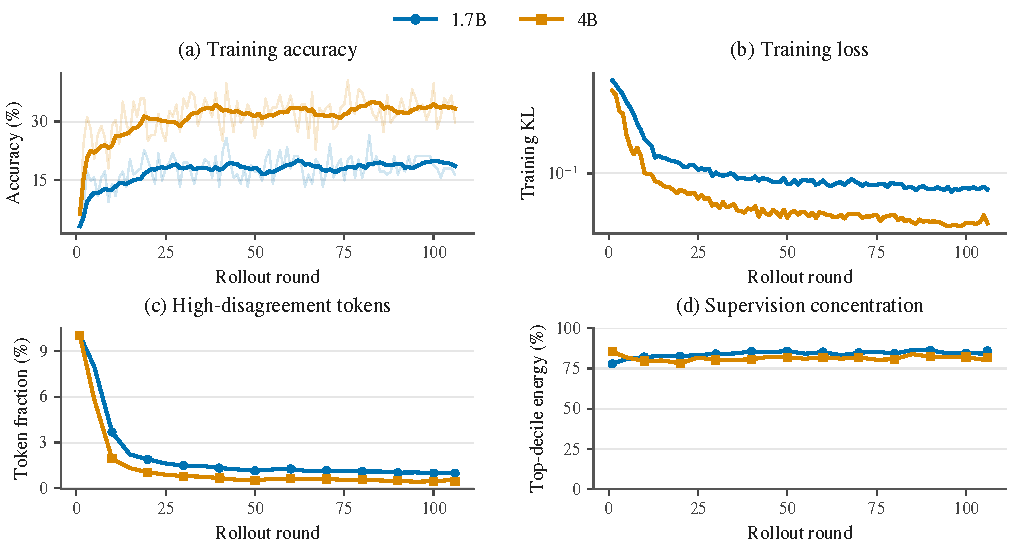
\includegraphics[width=\textwidth]{figures/dynamics.pdf}
 \caption{Training accuracy and supervision dynamics in the original two-scale FULL runs. (a) Accuracy on the 128 responses used for optimization, generated before each update. Light curves show raw accuracy; dark curves show the trailing 10-round mean. (b) Training KL. (c) Fraction of positions above the initial KL threshold. (d) Share of individual-token hidden-gradient energy contributed by the current highest-KL decile. Panels (b--d) show raw training observations.}
 \label{fig:dynamics}
\end{figure*}
\begin{table}[t]
\centering
\caption{Training dynamics of FULL. $\|g_\theta\|$ is the parameter gradient norm before clipping; hidden RMS aggregates individual token gradients. High frequency uses the fixed initial KL threshold. KL-top is the gradient-energy share of the current highest-KL decile. Frequency and energy shares are percentages. Entries are initial / final (updates 1 / 106).}
\label{tab:dynamics}
\small
\setlength{\tabcolsep}{3pt}
\begin{tabular}{lrr}
\toprule
Metric & 1.7B & 4B \\
\midrule
Train accuracy (\%) & 3.13 / 16.41 & 6.25 / 29.69 \\
Training KL & 0.473 / 0.077 & 0.397 / 0.044 \\
$\|g_\theta\|$ & 9.808 / 0.556 & 6.874 / 0.258 \\
Hidden RMS & 0.774 / 0.244 & 0.505 / 0.125 \\
High frequency (\%) & 10.00 / 0.99 & 10.00 / 0.46 \\
KL-top energy (\%) & 77.85 / 85.99 & 85.57 / 81.83 \\
\bottomrule
\end{tabular}
\end{table}

\begin{table*}[!htbp]
\centering
\caption{Supervision in paired-study FULL at both scales. High is the percentage above the initial KL threshold (1.7B: $0.843653$; 4B: $0.644093$). KL-top is the full hidden-gradient energy share of the current highest-KL decile.}
\label{tab:two_scale_signal}
\small
\setlength{\tabcolsep}{3pt}
\begin{tabular}{llrrrr}
\toprule
Model & Step & KL & RMS & High (\%) & KL-top (\%) \\
\midrule
1.7B & 1 & 0.3848 & 0.7149 & 10.00 & 82.12 \\
1.7B & 10 & 0.1874 & 0.4218 & 5.92 & 82.32 \\
1.7B & 30 & 0.0984 & 0.2746 & 2.26 & 83.50 \\
1.7B & 60 & 0.0898 & 0.2672 & 1.92 & 84.14 \\
1.7B & 100 & 0.0755 & 0.2436 & 1.48 & 85.50 \\
1.7B & 106 & 0.0751 & 0.2397 & 1.47 & 84.69 \\
4B & 1 & 0.3208 & 0.4469 & 10.00 & 87.43 \\
4B & 10 & 0.1025 & 0.1986 & 3.41 & 79.36 \\
4B & 30 & 0.0637 & 0.1568 & 1.43 & 79.85 \\
4B & 60 & 0.0506 & 0.1366 & 1.07 & 81.67 \\
4B & 100 & 0.0431 & 0.1254 & 0.84 & 83.31 \\
4B & 106 & 0.0435 & 0.1238 & 0.79 & 81.87 \\
\bottomrule
\end{tabular}
\end{table*}

\paragraph{Mode-level signed coherence.}
For projected token gradients $a_t(x)=U^\top g_{h,t}(x)$ in the fixed early basis, let $v_j$ be a principal eigenvector of their second moment and $z_j(x)=v_j^\top a_t(x)$. We define $\kappa_j=(\mathbb E_x z_j)^2/\mathbb E_x z_j^2$ and average it over the stated modes. The statistic compares a signed mean with a second moment; its small values can reflect cancellation or heterogeneous magnitudes. This mode average differs from the space-aggregated coherence in Table~\ref{tab:space_coherence}.
\begin{figure*}[!htbp]
 \centering
 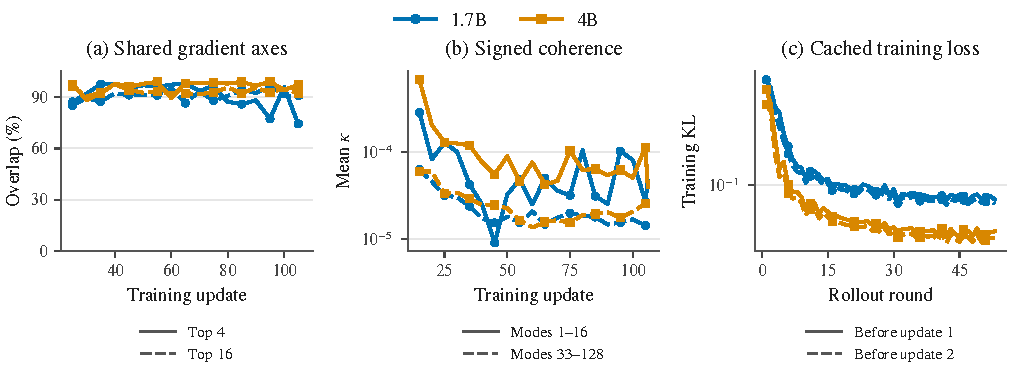
\includegraphics[width=\textwidth]{figures/utilization.pdf}
 \caption{Recurrent directions and residual fitting signal. Panels compare both scales through (a) leading demand-space overlap across recorded batches in the fixed early basis, (b) mode-averaged signed coherence, and (c) cached training KL before the first and second updates in equal-update reuse runs. Line samples and markers identify each series; the tail contains modes 33--128. The second curve measures residual loss after one update. The improvement produced by the second update is measured separately in Table~\ref{tab:reuse_summary}.}
 \label{fig:utilization}
\end{figure*}
\begin{table}[!htbp]
\centering
\caption{Second-update gains and component costs of reuse at equal update budget. Entries show FULL / reuse. Second-update training gains are multiplied by $10^3$ and averaged over six late readouts at cumulative updates $\geq60$; positive-gain counts cover all paired readouts. Actor time includes diagnostics; adjusted rows subtract them.}
\label{tab:reuse_summary}
\small
\setlength{\tabcolsep}{3pt}
\begin{tabular}{lrr}
\toprule
Measurement & 1.7B & 4B \\
\midrule
Second-update gain & -- / 5.686 & -- / 4.677 \\
Positive second gains & -- / 11 of 11 & -- / 11 of 11 \\
\midrule
Generation (min) & 93.6 / 46.0 & 86.1 / 43.9 \\
Teacher (min) & 24.6 / 12.3 & 24.4 / 12.2 \\
Actor (min) & 64.7 / 46.4 & 95.2 / 83.0 \\
Diagnostic (min) & 24.1 / 6.2 & 33.5 / 23.2 \\
Rounds excl. diag. (min) & 181.8 / 109.9 & 193.9 / 126.6 \\
Actor excl. diag. (min) & 40.5 / 40.1 & 61.7 / 59.7 \\
\bottomrule
\end{tabular}
\end{table}

\begin{table}[t]
\centering
\caption{Demand overlap and signed coherence in the fixed step-10 basis. Overlap is a percentage; mode-averaged coherence $\kappa$ is multiplied by $10^3$. Early and final denote updates 15 and 106. At the last observation the comparison is step 95 versus step 106.}
\label{tab:demand}
\small
\setlength{\tabcolsep}{3pt}
\begin{tabular}{lrr}
\toprule
Metric & 1.7B & 4B \\
\midrule
Final top-4 overlap (\%) & 74.89 & 97.25 \\
Final top-16 overlap (\%) & 89.06 & 92.99 \\
Early top-16 coherence & 0.284 & 0.673 \\
Final top-16 coherence & 0.047 & 0.039 \\
Early tail-96 coherence & 0.063 & 0.059 \\
Final tail-96 coherence & 0.014 & 0.023 \\
\bottomrule
\end{tabular}
\end{table}

\begin{table*}[!htbp]
\centering
\caption{Cross-batch geometry at both scales: four disjoint subsets and six pairs at each checkpoint. Param. is mean complete-parameter gradient cosine; Neg. is the percentage of negative pairs. Hidden gives the all-dimension mean-gradient cosine; axes columns give centered full-hidden eigenspace overlap.}
\label{tab:two_scale_batch}
\small
\setlength{\tabcolsep}{3pt}
\begin{tabular}{llrrrrrr}
\toprule
Model & Phase & Step & Param. & Neg. & Hidden & Axes-4 & Axes-128 \\
\midrule
1.7B & FULL & 10 & 0.7325 & 0.0 & 0.8977 & 0.9528 & 0.6284 \\
1.7B & FULL & 30 & 0.1100 & 0.0 & 0.3874 & 0.8411 & 0.5875 \\
1.7B & FULL & 60 & 0.0396 & 16.7 & 0.0944 & 0.7881 & 0.5776 \\
1.7B & FULL & 100 & 0.0828 & 0.0 & 0.2323 & 0.8895 & 0.5997 \\
4B & FULL & 10 & 0.7696 & 0.0 & 0.8891 & 0.9700 & 0.6283 \\
4B & FULL & 30 & 0.3346 & 0.0 & 0.6550 & 0.9553 & 0.5877 \\
4B & FULL & 60 & 0.1029 & 0.0 & 0.3434 & 0.8917 & 0.5869 \\
4B & FULL & 100 & 0.0596 & 0.0 & 0.2460 & 0.9471 & 0.5629 \\
\bottomrule
\end{tabular}
\end{table*}

\begin{table*}[!t]
\centering
\caption{Original-study FULL references for the $\dagger$ configurations in Tables~\ref{tab:benchmark_summary} and~\ref{tab:representation_time_summary}. Benchmark entries are Mean@8 (\%); time is total training-process minutes. }
\label{tab:reference_full}
\small
\setlength{\tabcolsep}{4pt}
\renewcommand{\arraystretch}{1.12}
\begin{tabular}{lrrrrrrrrr}
\toprule
Model & MATH500 & HMMT25 & HMMT26 & AIME26 & Minerva & Avg. & Rollouts & Updates & Minutes \\
\midrule
1.7B & 65.53 & 1.25 & 3.41 & 8.33 & 26.79 & 21.06 & 106 & 106 & 214.8 \\
4B & 80.28 & 6.67 & 12.12 & 12.92 & 39.94 & 30.38 & 106 & 106 & 234.6 \\
\bottomrule
\end{tabular}
\end{table*}

\begin{table*}[t]
\centering
\caption{Training time for FULL and Adaptive FULL, in minutes. Bold $\downarrow$/$\uparrow$ percentages indicate reduced/increased process time relative to FULL of the same scale; FULL is the reference. Process sums training subprocess wall times, including initialization, checkpointing, and diagnostics; model merge and all benchmark evaluations are excluded. The last two columns subtract recorded diagnostic time from logged round and actor time. For 1.7B Adaptive FULL, round timings cover 39 of 40 updates, so only complete process time is reported. Within-scale runtime and diagnostic differences affect these measurements.}
\label{tab:training_time_overview}
\small
\setlength{\tabcolsep}{3pt}
\begin{tabular}{llrrrrrr}
\toprule
Model & Configuration & Rollouts & Updates & Process & \shortstack{Time change\\vs. FULL} & \shortstack{Rounds excl.\\diag.} & \shortstack{Actor excl.\\diag.} \\
\midrule
1.7B & FULL & 106 & 106 & 214.8 & -- & 181.8 & 40.5 \\
1.7B & Adaptive FULL & 40 & 40 & 75.2 & \textbf{$\downarrow$ 65.0\%} & -- & -- \\
4B & FULL & 106 & 106 & 234.6 & -- & 193.9 & 61.7 \\
4B & Adaptive FULL & 50 & 50 & 121.6 & \textbf{$\downarrow$ 48.1\%} & 91.8 & 29.7 \\
\bottomrule
\end{tabular}
\end{table*}

\begin{table*}[!htbp]
\centering
\caption{Training costs at both scales. Total time includes warmup, basis discovery, and diagnostics; benchmark evaluation is excluded. Actor memory compares the FULL and Adapter phases. Whole-device peaks include teacher, rollout, and other processes.}
\label{tab:two_scale_adapter_cost}
\small
\setlength{\tabcolsep}{3pt}
\begin{tabular}{lrrrr}
\toprule
Measurement & 1.7B FULL & 1.7B Adapter & 4B FULL & 4B Adapter \\
\midrule
Total training (min) & 146.36 & 128.99 & 330.40 & 294.69 \\
Change relative to FULL & -- & $\boldsymbol{\downarrow 11.87\%}$ & -- & $\boldsymbol{\downarrow 10.81\%}$ \\
Actor peak GPU 0 (GiB) & 66.64 & 21.38 & 47.36 & 21.61 \\
Actor peak GPU 1 (GiB) & 66.48 & 23.60 & 47.22 & 21.69 \\
Whole-device sampled peak (GiB) & 75.01 & 74.97 & 48.83 & 74.83 \\
\bottomrule
\end{tabular}
\end{table*}

\begin{table*}[!t]
\centering
\caption{Final paired-study hidden-gradient spectra: entries show RMS / energy effective rank. The upper block compares full hidden space, $U$, and its complement in FULL. The lower block uses equal-count KL groups: 18,870 positions per group in 1.7B and 19,767 in 4B. Low-KL residuals have extremely small magnitude. Additional spectral measures and original-study results appear in Appendix~\ref{app:supplementary}.}
\label{tab:spectrum_summary}
\small
\setlength{\tabcolsep}{3pt}
\begin{tabular}{llrrr}
\toprule
Model & Phase / KL group & Full hidden & $U$ & $U^\perp$ \\
\midrule
1.7B & FULL & 0.2397 / 303.36 & 0.0980 / 46.13 & 0.2188 / 353.50 \\
4B & FULL & 0.1238 / 371.55 & 0.0482 / 40.24 & 0.1140 / 439.17 \\
\midrule
\multicolumn{5}{l}{\textit{Equal-count KL groups in final FULL}} \\
1.7B & High & 0.698 / 306.26 & 0.285 / 47.11 & 0.637 / 355.26 \\
1.7B & Middle & 0.105 / 177.35 & 0.0436 / 33.08 & 0.0951 / 209.33 \\
1.7B & Low & 1.55e-08 / 39.18 & 7.43e-09 / 22.06 & 1.36e-08 / 41.10 \\
4B & High & 0.354 / 383.28 & 0.136 / 42.20 & 0.327 / 446.54 \\
4B & Middle & 0.0591 / 213.17 & 0.0249 / 30.43 & 0.0536 / 259.95 \\
4B & Low & 5.98e-08 / 74.28 & 2.74e-08 / 21.70 & 5.32e-08 / 86.16 \\
\bottomrule
\end{tabular}
\end{table*}

\begin{table}[t]
\centering
\caption{Gradient strength and spectral spread. The nuclear norm is normalized by the square root of the number of token positions; effective rank is the entropy rank of normalized squared singular values. The available directional spectra cover the selected subspace for 1.7B and all three spaces for 4B. Cells report updates 15 / 106.}
\label{tab:ranks}
\small
\setlength{\tabcolsep}{3pt}
\begin{tabular}{lrr}
\toprule
Model / space & Nuclear norm & Effective rank \\
\midrule
1.7B $U$ & 1.103 / 0.862 & 47.61 / 46.72 \\
4B $U$ & 0.563 / 0.411 & 37.76 / 40.87 \\
4B Full & 5.056 / 3.689 & 342.51 / 366.13 \\
4B $U^\perp$ & 4.792 / 3.498 & 411.14 / 432.99 \\
\bottomrule
\end{tabular}
\end{table}

\begin{table}[t]
\centering
\caption{Final-step effective ranks in $U$ after matching token counts across high-, middle-, and low-KL groups. The groups are the top decile, middle 80\%, and bottom decile. Rank quantifies spectral spread.}
\label{tab:matched}
\small
\setlength{\tabcolsep}{3pt}
\begin{tabular}{lrrrr}
\toprule
Model & Tokens & High & Middle & Low \\
\midrule
1.7B & 19519 & 46.92 & 36.06 & 19.17 \\
4B & 20085 & 42.65 & 31.16 & 23.88 \\
\bottomrule
\end{tabular}
\end{table}

\begin{table*}[!htbp]
\centering
\caption{Final token-gradient spectra at both scales. Nuclear norm is divided by $\sqrt N$. Effective, stable, and participation ranks are $\exp(-\sum_jw_j\log w_j)$, $1/\max_jw_j$, and $1/\sum_jw_j^2$, with normalized squared singular values $w_j$. FULL uses its fixed step-10 observation basis.}
\label{tab:two_scale_ranks}
\small
\setlength{\tabcolsep}{3pt}
\begin{tabular}{lllrrrrr}
\toprule
Model & Phase & Space & RMS & Nuclear & Effective & Stable & Participation \\
\midrule
1.7B & FULL & Full & 0.2397 & 6.4185 & 303.36 & 15.13 & 89.26 \\
1.7B & FULL & $U$ & 0.0980 & 0.8507 & 46.13 & 8.55 & 24.48 \\
1.7B & FULL & $U^\perp$ & 0.2188 & 6.0101 & 353.50 & 15.01 & 107.14 \\
4B & FULL & Full & 0.1238 & 3.6852 & 371.55 & 15.48 & 97.47 \\
4B & FULL & $U$ & 0.0482 & 0.4040 & 40.24 & 7.93 & 20.59 \\
4B & FULL & $U^\perp$ & 0.1140 & 3.4948 & 439.17 & 14.78 & 117.46 \\
\bottomrule
\end{tabular}
\end{table*}

\begin{table}[!htbp]
\centering
\caption{Gradient coherence within and outside the early displacement subspace in FULL. The fixed rank-128 basis $U$ is obtained from cumulative displacement through step 10. For $S\in\{U,U^\perp\}$, coherence is $C_S=\|\mathbb E[g_S]\|^2/\mathbb E[\|g_S\|^2]$, where $g_S$ is the projected token-level hidden gradient and expectations average tokens within a subset. Each entry averages the coherence of four disjoint training subsets. Coherence columns are multiplied by $10^3$; the final column is the ratio of their arithmetic means.}
\label{tab:space_coherence}
\small
\setlength{\tabcolsep}{8pt}
\begin{tabular}{llrrr}
\toprule
Model & Step & $C_U\ (\times10^3)$ & $C_{U^\perp}\ (\times10^3)$ & $C_U/C_{U^\perp}$ \\
\midrule
\multirow{4}{*}{1.7B} & 10 & 1.541510 & 0.636129 & $2.42\times$ \\
 & 30 & 0.083452 & 0.072830 & $1.15\times$ \\
 & 60 & 0.048085 & 0.046732 & $1.03\times$ \\
 & 100 & 0.060013 & 0.053196 & $1.13\times$ \\
\midrule
\multirow{4}{*}{4B} & 10 & 0.724922 & 0.335759 & $2.16\times$ \\
 & 30 & 0.214490 & 0.116319 & $1.84\times$ \\
 & 60 & 0.067903 & 0.057403 & $1.18\times$ \\
 & 100 & 0.073859 & 0.055186 & $1.34\times$ \\
\bottomrule
\end{tabular}
\par\smallskip
\begin{minipage}{0.96\textwidth}\footnotesize
This space-aggregated statistic measures the squared norm of the mean gradient relative to total gradient energy. The mode-averaged signed coherence in Table~\ref{tab:demand} instead averages the ratios for individual axes; cross-batch cosine compares mean-gradient directions between subsets. A lower $C_S$ can reflect a smaller mean gradient relative to its variance. Coherence alone cannot identify gradient conflict or establish a causal effect on validation gains.
\end{minipage}
\end{table}


\begin{table*}[!t]
\centering
\caption{Training budgets and total time, including initialization, warmup, basis discovery within the run, and diagnostics; benchmark evaluation and merge are excluded. Reductions use FULL from the same study; $\dagger$ rows use the original-study references in Table~\ref{tab:reference_full}.}
\label{tab:representation_time_summary}
\small
\setlength{\tabcolsep}{4pt}
\renewcommand{\arraystretch}{1.12}
\begin{tabular}{llrrrr}
\toprule
Model & Method & Rollouts & Updates & Minutes & Reduction \\
\midrule
\multirow{5}{*}{\textbf{1.7B}} & Base & 0 & 0 & -- & -- \\
 & FULL & 106 & 106 & 146.36 & -- \\
 & Adaptive FULL$^{\dagger}$ & 40 & 40 & 75.2 & \textbf{$\downarrow$ 65.0\%} \\
 & Reuse$^{\dagger}$ & 53 & 106 & 118.6 & \textbf{$\downarrow$ 44.8\%} \\
 & Adapter & 106 & 106 & 128.99 & $\boldsymbol{\downarrow 11.87\%}$ \\
\midrule
\multirow{5}{*}{\textbf{4B}} & Base & 0 & 0 & -- & -- \\
 & FULL & 106 & 106 & 330.40 & -- \\
 & Adaptive FULL$^{\dagger}$ & 50 & 50 & 121.6 & \textbf{$\downarrow$ 48.1\%} \\
 & Reuse$^{\dagger}$ & 53 & 106 & 152.5 & \textbf{$\downarrow$ 35.0\%} \\
 & Adapter & 106 & 106 & 294.69 & $\boldsymbol{\downarrow 10.81\%}$ \\
\bottomrule
\end{tabular}
\end{table*}


\begin{table}[!htbp]
\centering
\caption{Paired FULL supervision at updates 1 / 106. High frequency uses each scale's fixed initial upper-decile KL threshold; KL-top is the full hidden-gradient energy share of the current highest-KL decile. Intermediate observations appear in Appendix~\ref{app:supplementary}.}
\label{tab:supervision_summary}
\small
\setlength{\tabcolsep}{3pt}
\begin{tabular}{lrr}
\toprule
Measurement & 1.7B & 4B \\
\midrule
Training KL & 0.3848 / 0.0751 & 0.3208 / 0.0435 \\
Hidden RMS & 0.7149 / 0.2397 & 0.4469 / 0.1238 \\
High frequency (\%) & 10.00 / 1.47 & 10.00 / 0.79 \\
KL-top energy (\%) & 82.12 / 84.69 & 87.43 / 81.87 \\
\bottomrule
\end{tabular}
\end{table}



\FloatBarrier
\clearpage
\subsection{Complete Temporal Views of Paired FULL}
\label{app:complete_trajectories}
These plots retain the paired FULL trajectories underlying the structural comparisons in the main text.
\begin{figure}[!htbp]
\centering
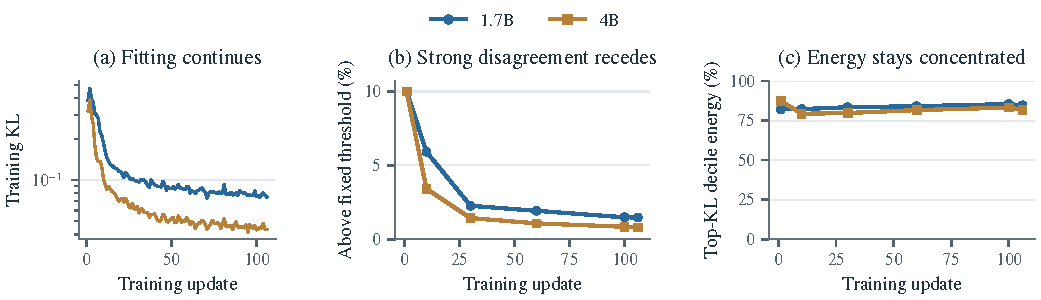
\includegraphics[width=.86\textwidth]{figures/full_trajectory_two_scale_dynamics.pdf}
\caption{Paired FULL training KL, fixed-threshold token frequency, and current top-KL decile energy throughout training. The energy trajectory complements the endpoint contribution bars in Figure~\ref{fig:two_scale_dynamics}.}
\label{fig:full_signal_trajectory}
\end{figure}

\begin{figure}[!htbp]
\centering
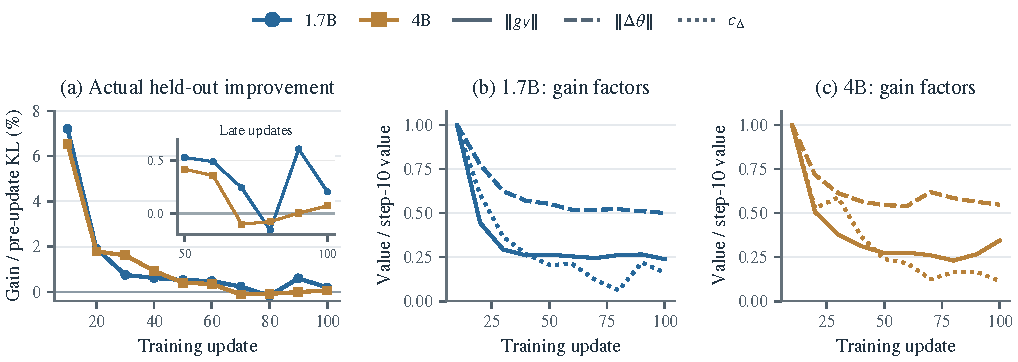
\includegraphics[width=.86\textwidth]{figures/full_trajectory_two_scale_transfer.pdf}
\caption{Relative actual held-out gains and complete normalized local-prediction factor trajectories from step 10 onward. These observations supplement the step-10/100 factor comparison in Figure~\ref{fig:two_scale_transfer}.}
\label{fig:full_update_trajectory}
\end{figure}

\clearpage

\end{document}


% This document was modified from the file originally made available by
% Pat Langley and Andrea Danyluk for ICML-2K. This version was created
% by Iain Murray in 2018, and modified by Alexandre Bouchard in
% 2019 and 2021 and by Csaba Szepesvari, Gang Niu and Sivan Sabato in 2022.
% Modified again in 2023 and 2024 by Sivan Sabato and Jonathan Scarlett.
% Previous contributors include Dan Roy, Lise Getoor and Tobias
% Scheffer, which was slightly modified from the 2010 version by
% Thorsten Joachims & Johannes Fuernkranz, slightly modified from the
% 2009 version by Kiri Wagstaff and Sam Roweis's 2008 version, which is
% slightly modified from Prasad Tadepalli's 2007 version which is a
% lightly changed version of the previous year's version by Andrew
% Moore, which was in turn edited from those of Kristian Kersting and
% Codrina Lauth. Alex Smola contributed to the algorithmic style files.
